\documentclass[11pt,a4paper]{article}

\usepackage[utf8]{inputenc}
\usepackage[T1]{fontenc}
\usepackage{lmodern}   % scalable fonts with complete glyphs in every viewer
\usepackage[english]{babel}
\usepackage[a4paper,margin=2.4cm]{geometry}

\usepackage{amsmath,amssymb}
\usepackage{graphicx}
\usepackage{booktabs}
\usepackage{array}
\usepackage{multirow}
\usepackage{caption}
\usepackage{subcaption}
\usepackage{xcolor}
\usepackage{enumitem}

\usepackage{algorithm}
\usepackage{algpseudocode}
\usepackage{float}
\floatstyle{ruled}
\restylefloat{algorithm}   % enables [H]: each pseudocode stays right below its description
\usepackage[hidelinks]{hyperref}

%--- Macros ---------------------------------------------------------------------
\newcommand{\code}[1]{\texttt{#1}}

\setlist{nosep,leftmargin=1.4em}
% lines with long \texttt (code identifiers): stretch them to avoid overfull boxes
% and tolerate the slight resulting slack without an underfull warning
\setlength{\emergencystretch}{3em}
\hbadness=3000

%==============================================================================
\title{\vspace{-1.2cm}\textbf{Generalized Assignment Problem (GAP)}\\[6pt]
       \normalsize Assignment of sellers to warehouses in first-mile logistics}
\author{Lucas Ojeda}
\date{}

%==============================================================================
\begin{document}
\maketitle
\vspace{-0.7cm}

%==============================================================================
\section{Introduction}
%==============================================================================
With the growth of e-commerce, logistics companies are trying to lower the costs of the
\emph{first mile}: moving the parcels from each seller to a reception point of the network. A
small seller gains nothing from scheduling a pickup visit, so the seller takes the parcels to a
\textbf{warehouse}: a shop of the network that, as a side activity, keeps them until the logistics
company collects them in consolidated form.

Today ThunderPack operates in a decentralized way: each seller chooses which warehouse to take the
parcels to and may change without notice. This makes inefficient use of the capacity of the
network, above all during demand peaks (Black Friday, Hot Sale), and causes complaints and extra
costs. ThunderPack is therefore considering a centralized mode, in which each seller is assigned a
fixed warehouse, respecting the capacities and minimizing the total distance traveled. The
business questions behind this work are:

\begin{itemize}
  \item \textbf{(Q1)} Is the capacity of the warehouse network enough, or does it need to be
        expanded to serve every seller?
  \item \textbf{(Q2)} Is there an assignment in which the sellers travel a reasonable distance?
  \item \textbf{(Q3)} Is a tool that delivers good solutions within \emph{a few minutes} viable,
        usable even in real time during demand peaks?
\end{itemize}

We model the problem as a \textbf{Generalized Assignment Problem} (GAP), which is NP-hard. The
work had two stages. In the first one we tackled the real scale ($n=1100$ sellers, $m=310$
warehouses) with heuristic methods: constructive heuristics, local search operators chained in a
VND and two metaheuristics that use it inside (ILS and LNS). Those solutions could only be compared
with each other: without a lower bound there was no way of knowing how far from the optimum they
were. In the second stage we added lower bounds (the linear and Lagrangian relaxations),
heuristics that start from those relaxations and exact methods on the SCIP solver. With them we
measured the true distance to the optimum on 57 benchmark instances and on the real one, and we
proved the optimum of 36 of them. In particular, the optimum of the real instance is $679.60$, and
the solver proves it in less than 10 seconds.

%==============================================================================
\section{Description of the model}
%==============================================================================
Let $N=\{1,\dots,n\}$ be the set of the $n$ sellers and $M=\{1,\dots,m\}$ that of the $m$
warehouses. Each warehouse $i\in M$ has capacity $b_i$. For a seller $j\in N$ and a warehouse
$i\in M$, $d_{ij}$ is the demand (units of capacity that $j$ takes up in $i$) and $c_{ij}$ the cost
of assigning $j$ to $i$ (at ThunderPack, the distance that $j$ would travel). We use binary
variables $x_{ij}=1$ if $j$ is assigned to $i$. The GAP in its general form is:
\begin{align}
  \min \quad & \sum_{i\in M}\sum_{j\in N} c_{ij}\,x_{ij} \label{eq:obj}\\
  \text{s.t.}\quad & \sum_{i\in M} x_{ij} = 1 && \forall\, j\in N \label{eq:asig}\\
  & \sum_{j\in N} d_{ij}\,x_{ij} \le b_i && \forall\, i\in M \label{eq:cap}\\
  & x_{ij}\in\{0,1\} && \forall\, i\in M,\ j\in N. \nonumber
\end{align}
Constraint \eqref{eq:asig} assigns each seller to exactly one warehouse and \eqref{eq:cap}
respects the capacities. Equivalently, a solution is a collection of disjoint sets
$\Gamma_1,\dots,\Gamma_m\subseteq N$, with $\Gamma_i$ the sellers assigned to $i$. In the real
instance the demand of a seller does not depend on the warehouse ($d_{ij}=d_j$); in the benchmark
ones it does.

\paragraph{Partial solutions and penalty.} Depending on the capacities and demands, there may be
no feasible assignment that covers every seller. In that case we admit \emph{partial solutions}
and penalize each unassigned seller. With $c_{max}=\max_{i\in M,\,j\in N} c_{ij}$ (the largest
possible distance) and $p=3\,c_{max}$, the objective function we evaluate is
\begin{equation}
  f(s)\;=\;\sum_{j \text{ assigned to } i(j)} c_{\,i(j)\,j}\;+\;p\cdot\bigl|\{j\in N:\ j\text{ unassigned}\}\bigr|.
  \label{eq:penal}
\end{equation}
The penalty $p$ per unassigned seller makes placing a seller in any warehouse always better than
leaving it out, without making infeasible the instances whose total capacity is not enough.
Adding a binary variable $u_j$ that indicates whether $j$ is left unassigned, \eqref{eq:penal} is
the objective of an integer model that a solver can solve directly (\S\ref{sec:exactos}), the
\textbf{compact model}:
\begin{align}
  \min \quad & \sum_{i\in M}\sum_{j\in N} c_{ij}\,x_{ij} + p\sum_{j\in N} u_j \label{eq:compacto}\\
  \text{s.t.}\quad & \sum_{i\in M} x_{ij} + u_j = 1 && \forall\, j\in N \label{eq:asigu}\\
  & \sum_{j\in N} d_{ij}\,x_{ij} \le b_i && \forall\, i\in M \nonumber\\
  & x_{ij},\,u_j\in\{0,1\} && \forall\, i\in M,\ j\in N. \nonumber
\end{align}

\paragraph{Interpretation as an assignment.} It is an assignment problem with capacities
(\emph{bin packing} with costs): the sellers are items with demand $d_{ij}$, the warehouses are
bins with capacity $b_i$, and assigning $j$ to $i$ costs $c_{ij}$. This guides the heuristics
(assign first what is closest or most urgent) and the local operators (move or exchange sellers
between warehouses). Moreover, choosing which sellers go to a given warehouse is a knapsack
problem: that structure is what the lower bounds and the exact methods exploit.

\paragraph{Data model (implementation).} The code mirrors the model: \code{Warehouse} (\code{id},
\code{capacity} $b_i$); \code{Seller} (\code{id}, \code{demand}, the vector of the $d_{ij}$, and
\code{distances}, a vector of pairs $(c_{ij},\,i)$ \textbf{sorted by increasing distance}, so that
the closest warehouses are tried first); \code{Solution} (the warehouse of each seller, the sellers
of each warehouse and the total cost, with methods \code{assign()} and \code{remove()}); and
\code{Instance} (warehouses, sellers, cost matrix and the penalty $p$; its constructor reads the
OR-Library format).


%==============================================================================
\section{Heuristic algorithms}
%==============================================================================
All the methods work on the same \code{Solution} representation and, except for the tabu search,
keep feasibility (\eqref{eq:cap}) at every step. We write $cap_i$ for the free capacity of
warehouse $i$ in the current solution.

\subsection{Constructive heuristics}
\paragraph{Nearest neighbor.} Goes through the sellers in order and assigns each one to its
closest feasible warehouse, taking advantage of \code{distances} being already sorted. If no
warehouse has capacity left, the seller is left unassigned. The first sellers take the best
warehouses and the last ones may find no room.

\begin{algorithm}[H]
\caption{Constructive heuristic: nearest neighbor}
\begin{algorithmic}[1]
\Function{NearestNeighbor}{$\mathrm{inst}$}
  \State $cap_i \gets b_i\ \forall i$;\quad $sol \gets$ empty;\quad $f \gets 0$
  \For{each seller $j\in N$ in order}
    \State $assigned \gets$ false
    \ForAll{$(dist,i)$ in $distances_j$ (increasing)}
      \If{$cap_i \ge d_{ij}$}
        \State assign $j$ to $i$;\ \ $f \mathrel{+}= dist$;\ \ $cap_i \mathrel{-}= d_{ij}$;\ \ $assigned\gets$ true;\ \ \textbf{break}
      \EndIf
    \EndFor
    \If{\textbf{not} $assigned$}\ $f \mathrel{+}= p$\ \EndIf
  \EndFor
  \State \Return $sol$
\EndFunction
\end{algorithmic}
\end{algorithm}

\paragraph{Regret insertion.} At each step, for each unassigned seller it computes its best and
second-best feasible warehouse according to a \emph{desirability measure} $f_{ij}$ (lower is
better); the regret is the difference between both values (or $\infty$ if only one is feasible).
It assigns the seller with the largest regret to its best warehouse. The idea is to serve first
whoever loses the most by not taking its best option now, so as to reduce the bad assignments
forced at the end. With $f_{ij}=c_{ij}$ it is the classic regret insertion; following Martello and
Toth~\cite{martello1981} we also tried $f_{ij}=d_{ij}$ (\emph{demand}) and $f_{ij}=d_{ij}/b_i$
(\emph{relative demand}), which fill the warehouses more slowly. On the instances with tight
capacity this matters: guided by the cost, the constructive heuristics leave thousands of sellers
unassigned (E1). The \emph{best constructive} solution is the best of the four.

\begin{algorithm}[H]
\caption{Constructive heuristic: regret insertion with measure $f$}
\begin{algorithmic}[1]
\Function{RegretInsertion}{$\mathrm{inst}$, $f$}
  \State $cap_i \gets b_i\ \forall i$;\quad $sol \gets$ empty;\quad every $j$ unassigned
  \While{some unassigned $j$ has a feasible warehouse}
    \State for each unassigned $j$: $p^1_j$ ($p^2_j$) $=$ value $f_{ij}$ of its best (second-best) feasible warehouse
    \State $regret_j \gets p^2_j - p^1_j$\ \ (or $\infty$ if it has only one feasible warehouse)
    \State choose $j^\star = \arg\max_j regret_j$;\ assign it to its best warehouse;\ update $cap$ and the cost
  \EndWhile
  \State penalize the $j$ left unassigned
  \State \Return $sol$
\EndFunction
\end{algorithmic}
\end{algorithm}

\subsection{Local search operators}

\paragraph{Relocate multiple.} Generalized operator: moves up to $q$ convenient sellers from a
warehouse $i$ to another warehouse $k$ (those with the largest saving that fit in the free
capacity of $k$). The case $q{=}1$ is the simple relocate: move a single seller $j$, with cost
change $\Delta = c_{kj}-c_{ij}$, accepted if $c_{kj}<c_{ij}$ and $d_{kj}\le cap_k$. It is one of
the two main operators chained by the VND.

\begin{algorithm}[H]
\caption{\emph{Relocate multiple} operator (first improvement)}
\begin{algorithmic}[1]
\Function{RelocateMultiple}{$sol,\mathrm{inst},q$}
  \ForAll{pair of warehouses $(i,k)$ with $i\neq k$}
    \State $move \gets$ up to $q$ sellers of $\Gamma_i$ with $c_{kj}<c_{ij}$, those with the largest saving $c_{ij}-c_{kj}$, that fit in $cap_k$
    \If{$move\neq\emptyset$}
      \State move each $j\in move$ from $i$ to $k$;\ \ update $f$;\ \ \Return true
    \EndIf
  \EndFor
  \State \Return false
\EndFunction
\end{algorithmic}
\end{algorithm}

\paragraph{Swap multiple.} Generalized operator: applies up to $q$ successive exchanges (the best
feasible pair each time) between a pair of warehouses $i_1,i_2$. The case $q{=}1$ is the simple
swap: exchange two sellers $j_1\in\Gamma_{i_1}$ and $j_2\in\Gamma_{i_2}$, with cost change
$\Delta = (c_{i_2 j_1}+c_{i_1 j_2})-(c_{i_1 j_1}+c_{i_2 j_2})$, accepted if $\Delta<0$ and the
exchange respects both capacities. It is the other main operator of the VND.

\begin{algorithm}[H]
\caption{\emph{Swap multiple} operator (first improvement)}
\begin{algorithmic}[1]
\Function{SwapMultiple}{$sol,\mathrm{inst},q$}
  \ForAll{pair of warehouses $(i_1,i_2)$ with $i_1<i_2$}
    \State $done \gets 0$
    \While{$done < q$ \textbf{and} there is a feasible exchange with $\Delta<0$}
      \State apply the pair $j_1\in\Gamma_{i_1},\,j_2\in\Gamma_{i_2}$ with the smallest $\Delta=(c_{i_2 j_1}+c_{i_1 j_2})-(c_{i_1 j_1}+c_{i_2 j_2})$;\ update $cap$, $f$;\ $done \mathrel{+}= 1$
    \EndWhile
    \If{$done>0$}\ \Return true\ \EndIf
  \EndFor
  \State \Return false
\EndFunction
\end{algorithmic}
\end{algorithm}

Both generalized operators apply a fixed acceptance strategy (they scan the pairs and keep the
first one that improves, choosing the best moves within it): they have no first/best variant. That
distinction does exist in the \emph{simple versions} ($q{=}1$, a single seller / a single pair),
which we implemented separately with two acceptance criteria: \emph{first improvement} (applies the
first improving move) and \emph{best improvement} (explores the whole neighborhood and applies the
move with the largest gain). In E2 (\S\ref{sec:exp}) we compare the simple versions (first vs
best) against the two generalized operators; the VND chains the latter in first improvement.

\paragraph{Auxiliary operators for tight instances.} When capacity is scarce and some sellers are
left unassigned, the previous moves are not always enough. We implemented:
\begin{itemize}
  \item \code{assign\_unassigned}: tries to place each unassigned seller in its closest feasible
        warehouse.
  \item \code{assign\_with\_ejection}: to place an unassigned seller $j$ in a warehouse $k$
        without room, it ejects a seller $x$ from $k$ and relocates it to another warehouse $k'$
        with capacity, if the cost balance is favorable.
  \item \emph{cyclic exchange} (\code{cyclic\_exchange}): rotates three sellers among three
        warehouses ($j_1\to i_2$, $j_2\to i_3$, $j_3\to i_1$), freeing room through a cyclic
        rearrangement that \emph{relocate} and \emph{swap} (limited to two warehouses) cannot
        reach. To keep it tractable, the target warehouses are restricted to the 5 closest ones of
        each seller and first improvement is applied. It is decisive when capacity is scarce and
        all the nearby warehouses are full, so that no move between two warehouses can descend.
\end{itemize}

\subsection{Metaheuristics: VND, ILS and LNS}
\paragraph{VND (Variable Neighborhood Descent).} Chains all the local search neighborhoods: it
applies each one until it is exhausted, in a fixed order, and repeats the whole cycle while any of
them improved, until reaching a local optimum with respect to every neighborhood. The implemented
version goes through, in first improvement: \code{assign\_unassigned}, ejection, the two main
operators \emph{relocate multiple} and \emph{swap multiple} ($q{=}1\dots10$) and the
\emph{cyclic exchange} of 3 warehouses. It is the local improvement subroutine used by both
metaheuristics.

\begin{algorithm}[H]
\caption{Metaheuristic: VND (Variable Neighborhood Descent)}
\begin{algorithmic}[1]
\Function{VND}{$sol,\mathrm{inst}$}
  \State $improved \gets$ true
  \While{$improved$}
    \State $improved \gets$ false
    \While{\textsc{AssignUnassigned}($sol$)}\ $improved \gets$ true\ \EndWhile
    \While{\textsc{Ejection}($sol$)}\ $improved \gets$ true\ \EndWhile
    \For{$q = 1$ \textbf{to} $10$}
      \While{\textsc{RelocateMultiple}($sol$,$q$)}\ $improved \gets$ true\ \EndWhile
      \While{\textsc{SwapMultiple}($sol$,$q$)}\ $improved \gets$ true\ \EndWhile
    \EndFor
    \While{\textsc{CyclicExchange}($sol$)}\ $improved \gets$ true\ \EndWhile
  \EndWhile
\EndFunction
\end{algorithmic}
\end{algorithm}

\paragraph{ILS (Iterated Local Search).} Starts from the best constructive solution, already
improved with VND. At each iteration it copies the best solution and perturbs it: it applies
\code{strength} random feasible moves between warehouses (half \emph{swaps} and half
\emph{relocations}) to escape from the local optimum. Then it evaluates it again, applies VND and
keeps the best. Parameters: \code{strength}, seed and time budget, which includes the construction
and the VND of the initial solution.

\begin{algorithm}[H]
\caption{Metaheuristic: ILS (Iterated Local Search)}
\begin{algorithmic}[1]
\Function{ILS}{$\mathrm{inst}$, strength, seed, seconds}
  \State $best \gets$ \textsc{BestConstructive};\ \ \textsc{VND}($best$);\ \ evaluate $f(best)$
  \While{elapsed time $<$ seconds}
    \State $s \gets best$;\ \ \textsc{Perturb}($s$, strength)\ \small{[half random \textit{swaps}, half random \textit{relocations}]}
    \State evaluate $f(s)$;\ \ \textsc{VND}($s$)
    \If{$f(s) < f(best)$}\ $best \gets s$\ \EndIf
  \EndWhile
  \State \Return $best$
\EndFunction
\end{algorithmic}
\end{algorithm}

\paragraph{LNS (Large Neighborhood Search / \emph{ruin-and-recreate}).} Same structure, but with a
larger perturbation: at each iteration it unassigns \code{destroy} random sellers (\emph{ruin}) and
lets the VND reinsert and reoptimize them (\emph{recreate}), accepting only if it improves. By
rebuilding a part of the solution from scratch, LNS can rearrange assignments that ILS, tied to
local moves, does not reach. Parameters: \code{destroy}, seed and time budget; it can also start
from a given solution (E9).

\begin{algorithm}[H]
\caption{Metaheuristic: LNS (Large Neighborhood Search)}
\begin{algorithmic}[1]
\Function{LNS}{$\mathrm{inst}$, destroy, seed, seconds}
  \State $best \gets$ \textsc{BestConstructive} (or a given solution);\ \ \textsc{VND}($best$);\ \ evaluate $f(best)$
  \While{elapsed time $<$ seconds}
    \State $s \gets best$;\ \ unassign \textit{destroy} random sellers of $s$\ \small{[\textit{ruin}]}
    \State \textsc{VND}($s$);\ \ evaluate $f(s)$\ \small{[\textit{recreate}]}
    \If{$f(s) < f(best)$}\ $best \gets s$\ \EndIf
  \EndWhile
  \State \Return $best$
\EndFunction
\end{algorithmic}
\end{algorithm}

\subsection{Tabu search}
On the tightest instances every improvement first needs to free room in a full warehouse, and a
search that never leaves the feasible region gets stuck. Inspired by Yagiura, Ibaraki and
Glover~\cite{yagiura2004}, we implemented a tabu search that allows exceeding the capacities for a
while, charging a penalty for each unit of excess. That is, it minimizes
\[
  \tilde f(s) \;=\; f(s) + \sum_{i\in M} \alpha_i \max\Bigl(0,\ \sum_{j\in\Gamma_i} d_{ij} - b_i\Bigr),
\]
where the weight $\alpha_i$ of each warehouse adjusts itself: it grows by 5\,\% at each iteration
in which the warehouse is overloaded, and all of them shrink by 2\,\% when the solution becomes
feasible again. Besides moving and exchanging sellers, it uses \emph{ejection chains}: a seller
enters a warehouse and pushes another one out to a third. So as not to undo right away what it
did, a seller cannot return for some iterations to the warehouse it left.

%==============================================================================
\section{Lower bounds and exact methods}\label{sec:exactos}
%==============================================================================
A \textbf{lower bound} $LB$ is a value that no solution can beat. It serves two purposes: measuring
the \emph{true gap} of a solution, $(f(s)-LB)/LB$, and discarding parts of the problem that only
lead to solutions worse than the best known one. When a solution reaches the bound, it is optimal.

\subsection{Linear relaxation and roundings}
If \emph{fractions} of sellers may be assigned, that is, if $x_{ij},u_j\in\{0,1\}$ is replaced by
$x_{ij},u_j\in[0,1]$ in \eqref{eq:compacto}, the model becomes a linear program (LP), which is
solved quickly and gives a lower bound. Its solution has a useful property (Benders and van
Nunen~\cite{benders1983}): the LP has $n+m$ constraints, so its basic solution has at most $n+m$
positive variables, and since each seller needs at least one, at most $m$ sellers are split among
several warehouses. That gives a simple heuristic, the \emph{LP rounding}: the integral sellers
keep their warehouse, the split ones are inserted where they fit and then the VND is applied.

We also tried the rounding of Shmoys and Tardos~\cite{shmoys1993}, which from the LP solution $x^*$
builds an assignment with
\[
  \text{cost} \;\le\; \text{LP bound}
  \qquad\text{and}\qquad
  \sum_{j\in\Gamma_i} d_{ij} \;\le\; b_i + \max_{j:\,x^*_{ij}>0} d_{ij}\quad \forall\, i\in M,
\]
that is, with a guaranteed cost but possibly exceeding the capacities. And we tried two families
of \emph{cutting planes} (inequalities added to the LP to bring it closer to the integer problem).
The first are the cover inequalities: if a set $C$ of sellers does not fit in warehouse $i$
($\sum_{j\in C} d_{ij} > b_i$), at most $|C|-1$ of them can go to $i$,
\[
  \sum_{j\in C} x_{ij} \;\le\; |C|-1
\]
(in the implementation, extended to the sellers heavier than those of $C$). The second is an exact
separation, which looks for the most violated valid inequality for the knapsack of each warehouse
(Avella, Boccia and Vasilyev~\cite{avella2010}).

\subsection{Lagrangian relaxation}
The other way of relaxing the problem is to allow a seller to end up in no warehouse or in several,
charging it a price $\lambda_j$ for each violation of \eqref{eq:asigu} (Fisher, Jaikumar and Van
Wassenhove~\cite{fisher1986}). Without that constraint, the problem splits into one knapsack
problem per warehouse: which sellers to fill it with, according to their costs and the prices. For
each set of prices $\lambda$,
\begin{align*}
  L(\lambda) &\;=\; \sum_{j\in N}\lambda_j \;-\; \sum_{i\in M} KP_i(\lambda) \;+\; \sum_{j\in N}\min(0,\ p-\lambda_j),\\
  KP_i(\lambda) &\;=\; \max\Bigl\{\sum_{j\in N} (\lambda_j-c_{ij})\,x_j \;:\; \sum_{j\in N} d_{ij}\,x_j\le b_i,\ x\in\{0,1\}^n\Bigr\},
\end{align*}
is a lower bound. The \emph{subgradient method} keeps adjusting the prices: it raises that of the
sellers that ended up in no warehouse and lowers that of those that ended up in several. With
$g_j = 1-\sum_i x_{ij}-u_j$ (the violation of each seller in the solution of the knapsacks) and $UB$
the cost of the best known solution, the step is
\[
  \lambda \;\gets\; \lambda + t\,g, \qquad t \;=\; \mu\,\frac{UB - L(\lambda)}{\|g\|^2},
\]
with $\mu$ starting at 2 and halved when the bound stops improving. This bound is much better than
the LP one (E7).

The knapsacks are, moreover, almost a solution. The \emph{Lagrangian heuristic} leaves each
repeated seller in the cheapest of its warehouses and inserts the missing ones; it turned out to be
one of the best starting points we found (E9, E10).

\subsection{Variable fixing}
With the Lagrangian prices one can compute, for each seller-warehouse pair, a bound on the best
possible cost if that seller goes to that warehouse. If $KP_i^{+j}$ and $KP_i^{-j}$ are the
knapsack of $i$ with $j$ forced in and forced out, that bound is
\[
  L^1_{ij} \;=\; \sum_{l\in N}\lambda_l - KP_i^{+j} - \sum_{k\neq i} KP_k^{-j} + \sum_{l\neq j}\min(0,\ p-\lambda_l),
\]
and that of the solutions that do \emph{not} assign $j$ to $i$ is $L^0_{ij} = L(\lambda) + KP_i -
KP_i^{-j}$. If $L^1_{ij}$ already exceeds the cost $UB$ of the best known solution (with integral
costs, if $L^1_{ij} > UB-1$), the pair is discarded: no better solution uses it; if $L^0_{ij}$ is
the one that exceeds it, $j$ is fixed to $i$. All these knapsacks come out of two dynamic programs,
one forward and one backward over the sellers, in the time of a single knapsack per warehouse. What
is left is a much smaller problem, and the better the known solution, the more pairs are discarded.
Since the solver finds better solutions during the search, we also implemented \emph{re-fixing}:
each time a better solution appears, the pairs are checked again and the new ones are discarded.
Posta, Ferland and Michelon~\cite{posta2012} use a similar idea to solve the GAP exactly.

\subsection{Exact methods}
\paragraph{Integer model in SCIP.} We solve the model directly with the SCIP solver~\cite{scip},
giving it the best heuristic solution as a starting point. We tried it alone, after the fixing (on
the reduced problem) and with re-fixing during the search.

\paragraph{Branch-and-price.} Instead of deciding seller by seller, this formulation chooses for
each warehouse a \emph{set} of sellers that fits in it (Savelsbergh~\cite{savelsbergh1997}). If each
column $s$ is a set of sellers that fits in warehouse $i(s)$, with cost $c_s=\sum_{j\in s}c_{i(s)j}$,
the problem is
\[
  \min \sum_s c_s\lambda_s + p\sum_j u_j
  \quad\text{s.t.}\quad
  \sum_{s\ni j}\lambda_s + u_j = 1\ \ (\pi_j),\qquad
  \sum_{s:\,i(s)=i}\lambda_s \le 1\ \ (\mu_i),\qquad
  \lambda_s,u_j\in\{0,1\}.
\]
Since there are too many sets to write them all, only the useful ones are generated: with the
duals $\pi$ of the linear program, the best new set of each warehouse is again a knapsack, with
profits $\pi_j-c_{ij}$ (\emph{column generation}). At each round,
$L(\pi)=\sum_j\min(\pi_j,p)-\sum_i KP_i(\pi)$ is a valid bound, and at the end it matches the best
Lagrangian bound. When the solution comes out fractional, it branches, that is, it splits the
problem in two (seller $j$ goes to warehouse $i$, or not). We added the usual techniques to speed
it up (stabilization, strong branching, a heuristic on the generated sets, among others) and the
fixing.

\paragraph{Bundle method.} On the large instances, the branch-and-price does not finish computing
the bound of the first node: the linear program that combines the sets is highly degenerate and the
simplex moves very slowly. We tried solving it with another linear solver (HiGHS~\cite{highs}, with
the simplex and with an interior point method) and with a \emph{bundle method}~\cite{briant2008},
which computes the same bound without solving that linear program. The method maximizes $L(\pi)$
step by step: at each step it solves, with the sets $B_i$ generated so far,
\[
  \max_\pi\ \sum_j\min(\pi_j,p) - \sum_i\max_{s\in B_i}\bigl(\pi(s)-c_s\bigr) - \frac{\|\pi-\hat\pi\|^2}{2t},
\]
where the last term prevents moving far from the best known point $\hat\pi$. If the new point
improves the bound enough, it becomes $\hat\pi$; if not, $t$ is reduced and it tries closer.

\subsection{Matheuristic and portfolio}
The \emph{MIP-LNS} is an LNS in which the solver does the reconstruction: at each iteration it frees
the sellers of a group of nearby warehouses and lets SCIP reassign them in the best possible way
(with a limit of 5\,s), with the rest fixed. Freeing whole warehouses allows exchanges among them
that the VND does not find. The \emph{portfolio} combines everything within the same budget: the LP
rounding and the Lagrangian heuristic, then the tabu search from the better of the two and, at the
end, the MIP-LNS.

%==============================================================================
\section{Implementation notes and difficulties}
%==============================================================================
\begin{itemize}
  \item \textbf{Build and usage.} Code in C++ (\code{c++17}). From \code{src/}, \code{make} builds
        \code{gap\_simulator} (ILS on one instance) and the test suite of the heuristics,
        \code{./tests <mode>}, with no external dependencies. The exact part uses SCIP and HiGHS,
        installed with \code{pixi install}; \code{make exact} builds \code{gap\_exact}, which runs
        any method on one instance (e.g., \code{./gap\_exact mipfix instances/real/real\_instance 60
        <output>} writes the optimal assignment of the real one), and \code{exact\_tests}, with the
        experiments E7--E17. The CSV files go to \code{src/results/} and the figures are generated
        with \code{python src/plots.py}.
  \item \textbf{Optimizations.} Distances presorted per seller (pairs $(c_{ij},i)$) to try the
        closest warehouses first; incremental evaluation of the cost by $\Delta$ in $O(1)$ per
        move; and dynamic programming for the knapsacks, which are solved thousands of times.
  \item \textbf{Correctness.} More than 4400 automated tests: feasibility and cost of every
        solution, the knapsack against enumeration, and every exact method against brute force on
        small random instances.
  \item \textbf{Unassigned sellers and feasibility.} Partial solutions and the penalty $p$ are
        central for the heuristics on the tight instances: guided by the cost, the constructive
        heuristics leave thousands of sellers unassigned.
  \item \textbf{Difficulties.} (i) On the large instances the bound of the branch-and-price cannot
        be completed with an LP (E14), which led to the bundle method. (ii) On the large type-$e$
        instances the VND of the initial solution takes longer than the whole budget of the
        metaheuristics (E3, E5). (iii) Integrating the fixing inside the solver required care with
        several details of SCIP; one of them made solutions already found get lost, and the tests
        caught it.
\end{itemize}

%==============================================================================
\section{Experiments}\label{sec:exp}
%==============================================================================
\subsection{Environment}
\begin{itemize}
  \item \textbf{Processor / RAM / OS:} AMD Ryzen 9 8945HX / 32\,GB / Linux.
  \item \textbf{Compiler and solvers:} g++ 16.2 (\code{-O2}); SCIP 10.1 and HiGHS 1.15.
  \item \textbf{Measurement:} \code{std::chrono} around each method. The heuristics and the local
        search are deterministic (one run); the metaheuristics are averaged over $R=5$ seeds and
        stopped by time according to the size ($2$/$10$/$60$\,s for $n\le200$ / $n\le900$ /
        larger). The exact methods have a limit of 600\,s (300\,s in E14--E16) and run several
        instances in parallel.
  \item \textbf{Reproducibility:} the experiments are automated in the programs \code{tests.cpp}
        and \code{exact\_tests.cpp} of \code{src/}; they produce the CSV files of
        \code{src/results/} and the figures.
\end{itemize}

\subsection{Instances}
We use the five benchmark groups of the GAP (Table~\ref{tab:grupos}): $a$ and $b$ from the
OR-Library~\cite{beasley1990}, and $c$, $d$ and $e$ from Yagiura's site (those of types $c$ and $d$
with $n\le200$ are the OR-Library ones), plus the real ThunderPack instance. In the real one the
total capacity is $15{,}235$ and the total demand $10{,}707$ (ratio $0.70$); the demands range from
5 to 19 units and the capacities from 20 to 250. Appendix~\ref{sec:apendice} gives the best bound
and the best solution of each instance.

\begin{table}[ht]
\centering
\caption{Instance groups: size and number of instances with the optimum proven at the end of the
work.}
\label{tab:grupos}
\small
\begin{tabular}{l r r r l r}
\toprule
Group & Instances & $m$ & $n$ & Source & Optimum proven \\
\midrule
$a$ & 6  & 5--20 & 100--200  & OR-Library & 6 \\
$b$ & 6  & 5--20 & 100--200  & OR-Library & 6 \\
$c$ & 15 & 5--80 & 100--1600 & OR-Library and Yagiura & 10 \\
$d$ & 15 & 5--80 & 100--1600 & OR-Library and Yagiura & 2 \\
$e$ & 15 & 5--80 & 100--1600 & Yagiura & 11 \\
\textbf{real} & 1 & 310 & 1100 & ThunderPack & 1 \\
\midrule
Total & 58 & & & & 36 \\
\bottomrule
\end{tabular}
\end{table}

\subsection{Metrics}
\begin{itemize}
  \item \textbf{Cost} $f(s)$: objective function \eqref{eq:penal} (penalty included).
  \item \textbf{Unassigned}: number of sellers without a warehouse (measures feasibility, Q1).
  \item \textbf{Time} of execution (Q3).
  \item \textbf{True gap} $(f(s)-LB)/LB\cdot 100\%$ with respect to the \emph{best lower bound}
        $LB$ known for that instance (the best of all the relaxations and exact methods). If the
        best solution reaches $LB$, the optimum is proven.
\end{itemize}

\subsection{Research questions}
\begin{itemize}
  \item \textbf{(RQ1)} Which constructive heuristic gives the best starting point (quality and \%
        unassigned)?
  \item \textbf{(RQ2)} How much does each local search operator contribute, and first vs.\ best
        improvement?
  \item \textbf{(RQ3)} Does the VND improve over a single operator? Does the order of the
        neighborhoods matter?
  \item \textbf{(RQ4)} Which parameters of ILS (\code{strength}) and LNS (\code{destroy}) give the
        best quality/time trade-off, and how do both metaheuristics compare?
  \item \textbf{(RQ5)} Overall: constructive $\to$ VND $\to$ ILS/LNS, how much is gained and at
        what time cost, depending on the size of the instance?
  \item \textbf{(RQ6, real case)} What quality and time are obtained on the ThunderPack instance,
        and what does it imply for Q1--Q3?
  \item \textbf{(RQ7)} How far from the optimum are the heuristics, and how many instances do the
        exact methods solve?
  \item \textbf{(RQ8)} Is it worth starting the searches from the relaxations?
  \item \textbf{(RQ9)} Which bound is better, that of the cutting planes or the Lagrangian one? And
        which LP rounding?
  \item \textbf{(RQ10)} What limits the branch-and-price on the large instances?
  \item \textbf{(RQ11)} How much slack does the real network have?
  \item \textbf{(RQ12)} Can the instances still open be closed?
\end{itemize}

\subsection{E1 --- Constructive heuristics (RQ1)}
\emph{Hypothesis.} We expected the regret insertion to beat the nearest neighbor, by anticipating
the assignments forced at the end, and the demand-based measures to help on the tight instances.
The times of all four are negligible (at most $0.05$\,s).

\begin{table}[ht]
\centering
\caption{E1: mean true gap (\%) and total unassigned sellers of each constructive heuristic, by
group. NN: nearest neighbor; the other three are the regret insertion with $f_{ij}=c_{ij}$ (cost),
$d_{ij}$ (demand) and $d_{ij}/b_i$ (relative demand).}
\label{tab:const}
\small
\resizebox{\textwidth}{!}{%
\begin{tabular}{l r r r r r r r r r}
\toprule
 & & \multicolumn{2}{c}{NN} & \multicolumn{2}{c}{Regret, cost} & \multicolumn{2}{c}{Regret, demand} & \multicolumn{2}{c}{Regret, rel.\ demand}\\
\cmidrule(lr){3-4}\cmidrule(lr){5-6}\cmidrule(lr){7-8}\cmidrule(lr){9-10}
Group & Inst. & Gap & Unassigned & Gap & Unassigned & Gap & Unassigned & Gap & Unassigned \\
\midrule
$a$ & 6 & 1.30 & 0 & \textbf{0.01} & 0 & 109.55 & 0 & 109.55 & 0 \\
$b$ & 6 & 116.37 & 122 & 97.78 & 107 & \textbf{92.12} & 0 & \textbf{92.12} & 0 \\
$c$ & 15 & 203.84 & 1,779 & 202.53 & 1,782 & \textbf{109.15} & 0 & 140.71 & 0 \\
$d$ & 15 & 179.06 & 4,462 & 177.03 & 4,543 & \textbf{67.74} & 0 & 68.48 & 0 \\
$e$ & 15 & 1,561.17 & 6,622 & 1,606.73 & 6,837 & \textbf{692.45} & 0 & 692.84 & 0 \\
\textbf{real} & 1 & 15.98 & 0 & \textbf{5.65} & 0 & 15.98 & 0 & 496.09 & 0 \\
\bottomrule
\end{tabular}%
}
\end{table}

The results (Table~\ref{tab:const}) confirm the hypothesis only in part. The cost-based insertion
wins in group $a$ (loose) and on the real instance, but on the tight groups the two cost-guided
constructive heuristics leave hundreds or thousands of sellers unassigned, and the penalty
dominates the cost. The demand-based measures assign every seller, at a higher cost, and are the
best option from $b$ to $e$. Even so, the starting point is very far from the optimum: between 52
and 692\,\% on average in those groups.

\subsection{E2 --- Local search operators (RQ2)}
\emph{Hypothesis.} We expected \emph{best improvement} to reduce the cost more per sweep than
\emph{first} (at a higher time cost) and the generalized operators to add something over the simple
ones. Starting from three constructive heuristics (nearest neighbor, regret by cost and by demand)
we applied each operator until a local optimum on the 58 instances.

\begin{table}[ht]
\centering
\caption{E2: improvement (\%) over the cost of the constructive solution depending on which one it
starts from, largest improvement, mean time and mean number of passes (these three over all the
runs). The \emph{multiple} operators apply a fixed strategy ($q{=}1\dots10$), with no first/best
variant.}
\label{tab:bl}
\small
\resizebox{\textwidth}{!}{%
\begin{tabular}{l r r r r r r}
\toprule
 & \multicolumn{3}{c}{Mean improvement (\%) from} & & & \\
\cmidrule(lr){2-4}
Operator & NN & Regret, cost & Regret, demand & Max improvement (\%) & Mean time (s) & Mean passes \\
\midrule
relocate (first)   & 0.00 & 0.00 & 36.55 & 58.91 & 0.004 & 240.1 \\
relocate (best)    & 0.00 & 0.00 & 37.74 & 56.05 & 0.010 & 78.7 \\
swap (first)       & 1.70 & 0.70 & \textbf{48.01} & 79.10 & 0.143 & 614.2 \\
swap (best)        & 1.34 & 0.62 & 38.35 & 55.00 & 0.270 & 82.6 \\
\midrule
relocate multiple  & 0.00 & 0.00 & 38.04 & 67.11 & 0.004 & 221.6 \\
swap multiple      & 1.48 & 0.70 & 44.50 & 78.33 & 0.095 & 320.0 \\
\bottomrule
\end{tabular}%
}
\end{table}

The result (Table~\ref{tab:bl}) depends on the starting point. From the nearest neighbor and the
cost-based insertion, no \emph{relocate} improves, because those constructive heuristics already
assign each seller to its cheapest feasible warehouse; all the work is done by the \emph{swap}, and
it is little. From the demand-based regret, which assigns every seller but at a high cost, all the
operators improve a lot (between 36 and 48\,\%). In the \emph{swap}, \emph{first improvement}
improves more than \emph{best} ($48.0$ against $38.4\,\%$) and in half the time: accepting right
away leaves more room for the following moves. Used alone, the multiple operators stay close to the
simple ones; their advantage shows up when they are combined in the VND (E3).

\subsection{E3 --- VND vs.\ single operators (RQ3)}
\emph{Hypothesis.} We expected the VND, by combining neighborhoods, to beat any single operator,
above all on the tight instances. We start from the best constructive solution and compare simple
\emph{relocate} and \emph{swap}, a VND that chains only those two, and the full VND.

\begin{table}[ht]
\centering
\caption{E3: mean true gap (\%) of the final solution, from the best constructive solution, and
time of the full VND (mean and maximum), by group.}
\label{tab:vnd}
\small
\resizebox{\textwidth}{!}{%
\begin{tabular}{l r r r r r r r}
\toprule
Group & Constructive & Relocate & Swap & VND reloc.+swap & Full VND & Mean $t$ (s) & Max $t$ (s) \\
\midrule
$a$ & 0.01 & 0.01 & 0.01 & 0.01 & 0.01 & 0.01 & 0.02 \\
$b$ & 52.92 & 28.28 & 18.31 & 16.03 & \textbf{3.01} & 0.02 & 0.07 \\
$c$ & 109.15 & 25.36 & 10.89 & 4.75 & \textbf{3.73} & 3.26 & 27.93 \\
$d$ & 66.36 & 13.59 & 9.46 & 9.09 & \textbf{5.10} & 6.03 & 47.43 \\
$e$ & 691.59 & 431.01 & 162.74 & \textbf{160.33} & 218.56 & 39.07 & 382.73 \\
\textbf{real} & 5.65 & 5.65 & 3.65 & 3.08 & \textbf{2.34} & 0.37 & 0.37 \\
\bottomrule
\end{tabular}%
}
\end{table}

The data (Table~\ref{tab:vnd}) confirm the hypothesis in every group except $e$. The full VND
lowers the mean gap from 53 to 3\,\% in $b$, from 109 to 4\,\% in $c$ and from 66 to 5\,\% in $d$,
and on the real instance from $718$ to $695.5$, because the ejection and the \emph{3-cycle} place
sellers that the moves between two warehouses cannot relocate. In $e$, instead, it ends up worse
than the \emph{swap} alone and takes much longer (up to 383\,s): the order of the neighborhoods
matters, because each one changes the point from which the others continue.
Figure~\ref{fig:tiempo} shows how the time of the VND grows with the size.

\subsection{E4 --- Parameter tuning: ILS and LNS (RQ4)}
As the stopping criterion we use time (not the number of iterations), scaled by size: $2$\,s for
$n\le200$, $10$\,s for $n\le900$ and $60$\,s for the largest. Each configuration is averaged over 5
seeds. We tuned the \code{strength} of the ILS perturbation and the destruction size \code{destroy}
of the LNS on three representative instances.

\emph{Hypothesis.} ILS should be little sensitive to \code{strength} and LNS sensitive to
\code{destroy}. We expected comparable performance from both.

\begin{table}[ht]
\centering
\caption{Tuning: mean cost (5 seeds) by parameter value. Best per row in bold. Time limit: $2$\,s
(\code{b10200}), $10$\,s (\code{e15900}), $60$\,s (\code{real}). The optima are $2{,}827$,
$102{,}421$ and $679.60$.}
\label{tab:ils}
\small
\begin{tabular}{l r r r r}
\toprule
\multicolumn{5}{l}{\textit{ILS --- perturbation strength \code{strength}}}\\
Instance & $5$ & $10$ & $20$ & $40$ \\
\midrule
\code{b10200} & 2,845.0 & 2,843.0 & 2,841.2 & \textbf{2,836.2} \\
\code{e15900} & 420,850.0 & 420,454.2 & 419,350.0 & \textbf{419,334.6} \\
\code{real}   & 687.36 & 684.04 & 683.62 & \textbf{683.44} \\
\midrule
\multicolumn{5}{l}{\textit{LNS --- destruction size \code{destroy}}}\\
Instance & $20$ & $50$ & $100$ & \\
\midrule
\code{b10200} & \textbf{2,836.4} & 2,849.2 & 2,871.0 & \\
\code{e15900} & 419,333.8 & 418,982.6 & \textbf{417,722.6} & \\
\code{real}   & 686.80 & 682.80 & \textbf{682.42} & \\
\bottomrule
\end{tabular}
\end{table}

The hypothesis holds (Table~\ref{tab:ils}). ILS barely improves when the \code{strength} is raised
(40 is the best, but within one standard deviation of 20, which we kept), and LNS prefers to destroy
little on \code{b10200} and a lot on the large ones; we use 20 for $n\le900$ and 100 for the rest.
Both perform similarly. But on \code{e15900} both stay about four times above the optimum: the
10\,s budget is not even enough for the VND of the initial solution (29\,s in E3), and there the
configuration does not matter.

\begin{figure}[ht]
\centering
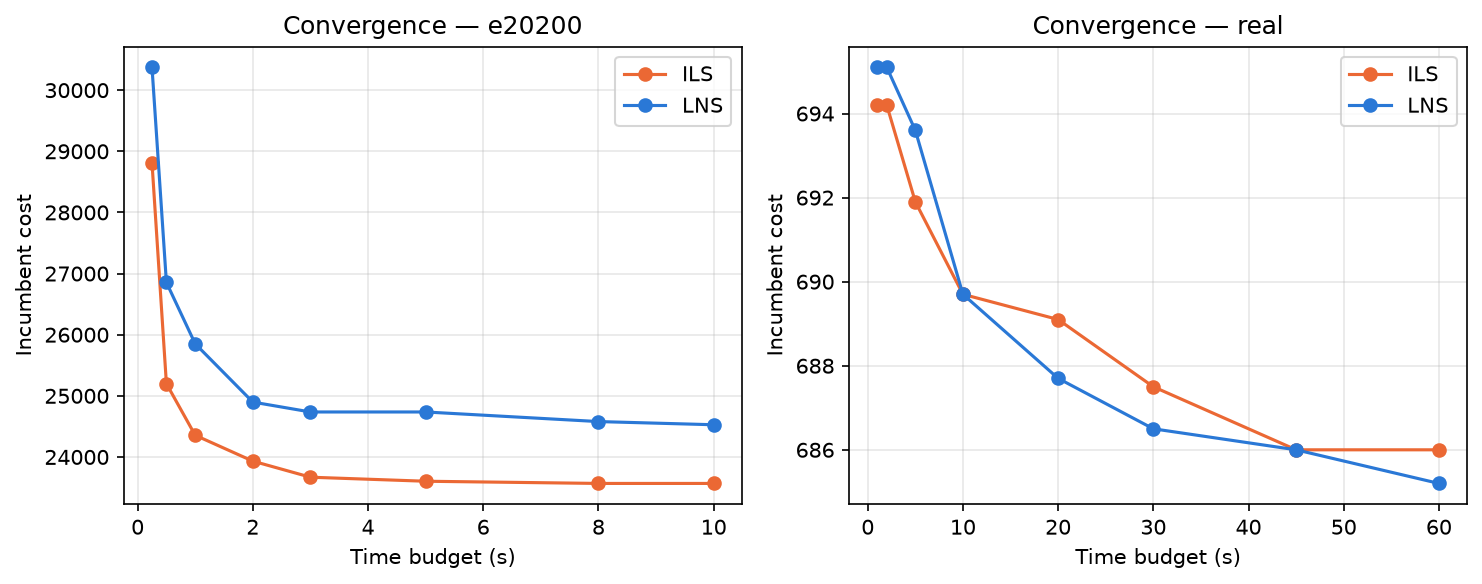
\includegraphics[width=0.92\linewidth]{figs/fig_convergence.png}
\caption{Convergence: incumbent cost vs.\ time budget, for ILS and LNS (seed 1), on a tight
instance (\code{e20200}, optimum $22{,}379$) and on the real one (optimum $679.60$).}
\label{fig:conv}
\end{figure}

\subsection{E5 --- Final comparison (RQ5)}
\emph{Hypothesis.} We expected quality to grow monotonically, constructive $<$ VND $<$
metaheuristic, with larger gains on the tight instances, and LNS to make the difference precisely
there. Table~\ref{tab:final} reports the mean true gap of each method by group.

\begin{table}[ht]
\centering
\caption{Final comparison: mean true gap (\%) by method and group (ILS and LNS: mean cost over 5
seeds). Mean time of the metaheuristic (limit according to size).}
\label{tab:final}
\small
\begin{tabular}{l r r r r r}
\toprule
Group & Constructive & VND & ILS & LNS & MH time (s) \\
\midrule
$a$ (avg.)    & 0.01 & 0.01 & \textbf{0.00} & 0.01 & 2.0 \\
$b$ (avg.)    & 52.92 & 3.01 & 0.33 & \textbf{0.31} & 2.0 \\
$c$ (avg.)    & 109.15 & 3.73 & 0.99 & \textbf{0.98} & 16.9 \\
$d$ (avg.)    & 66.36 & 5.10 & \textbf{2.85} & 2.98 & 16.8 \\
$e$ (avg.)    & 691.59 & 218.56 & \textbf{119.69} & 125.59 & 16.8 \\
\textbf{real} & 5.65 & 2.34 & 0.83 & \textbf{0.81} & 60.0 \\
\bottomrule
\end{tabular}
\end{table}

\begin{table}[ht]
\centering
\caption{ILS vs.\ LNS: cost over 5 seeds (best / worst / mean / standard deviation) on one instance
per group plus the real one, and the optimum. Lower is better; best mean cost per row in bold.}
\label{tab:ils_lns}
\small
\resizebox{\textwidth}{!}{%
\begin{tabular}{l r r r r r r r r r}
\toprule
 & & \multicolumn{4}{c}{ILS} & \multicolumn{4}{c}{LNS}\\
\cmidrule(lr){3-6}\cmidrule(lr){7-10}
Instance & Optimum & Best & Worst & Mean & Std.\ dev. & Best & Worst & Mean & Std.\ dev. \\
\midrule
a05100 & 1,698 & 1,698 & 1,698 & \textbf{1,698} & 0.00 & 1,698 & 1,698 & \textbf{1,698} & 0.00 \\
b10200 & 2,827 & 2,831 & 2,849 & 2,841.20 & 6.01 & 2,833 & 2,839 & \textbf{2,836.20} & 2.32 \\
e15900 & 102,421 & 423,256 & 423,279 & 423,263.20 & 8.47 & 423,216 & 423,272 & \textbf{423,254.40} & 20.49 \\
\textbf{real} & 679.60 & 683.70 & 686.90 & 685.26 & 1.17 & 683.70 & 686.90 & \textbf{685.12} & 1.06 \\
\bottomrule
\end{tabular}%
}
\end{table}

The progression constructive $\to$ VND $\to$ MH is monotonic in every group, but LNS does not make
the difference: ILS and LNS are on par (ILS has the better mean cost on 30 instances and LNS on 22;
Table~\ref{tab:ils_lns}). In $a$, $b$, $c$ and the real instance both stay below 1\,\% from the
optimum; in $d$, around 3\,\%; and in $e$, very far: on several of the large instances the VND of the
initial solution takes longer than the whole budget, and on the rest they stall. Without a lower
bound these distances could not be seen: against the best value found, the mean gap of the
metaheuristics did not exceed 9\,\% in any group (Figure~\ref{fig:gap}). Starting from the
relaxations corrects this (E9).

\begin{figure}[ht]
\begin{subfigure}{0.49\linewidth}
  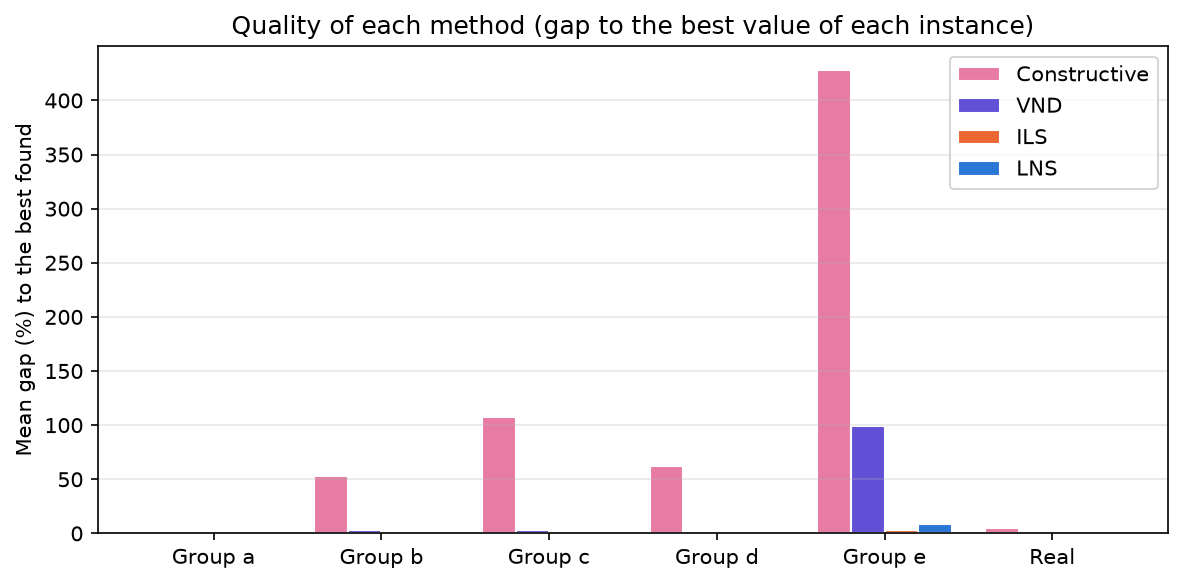
\includegraphics[width=\linewidth]{figs/fig_gap_method.png}
  \caption{Mean gap by method and group, against the best value found in E5.}\label{fig:gap}
\end{subfigure}\hfill
\begin{subfigure}{0.49\linewidth}
  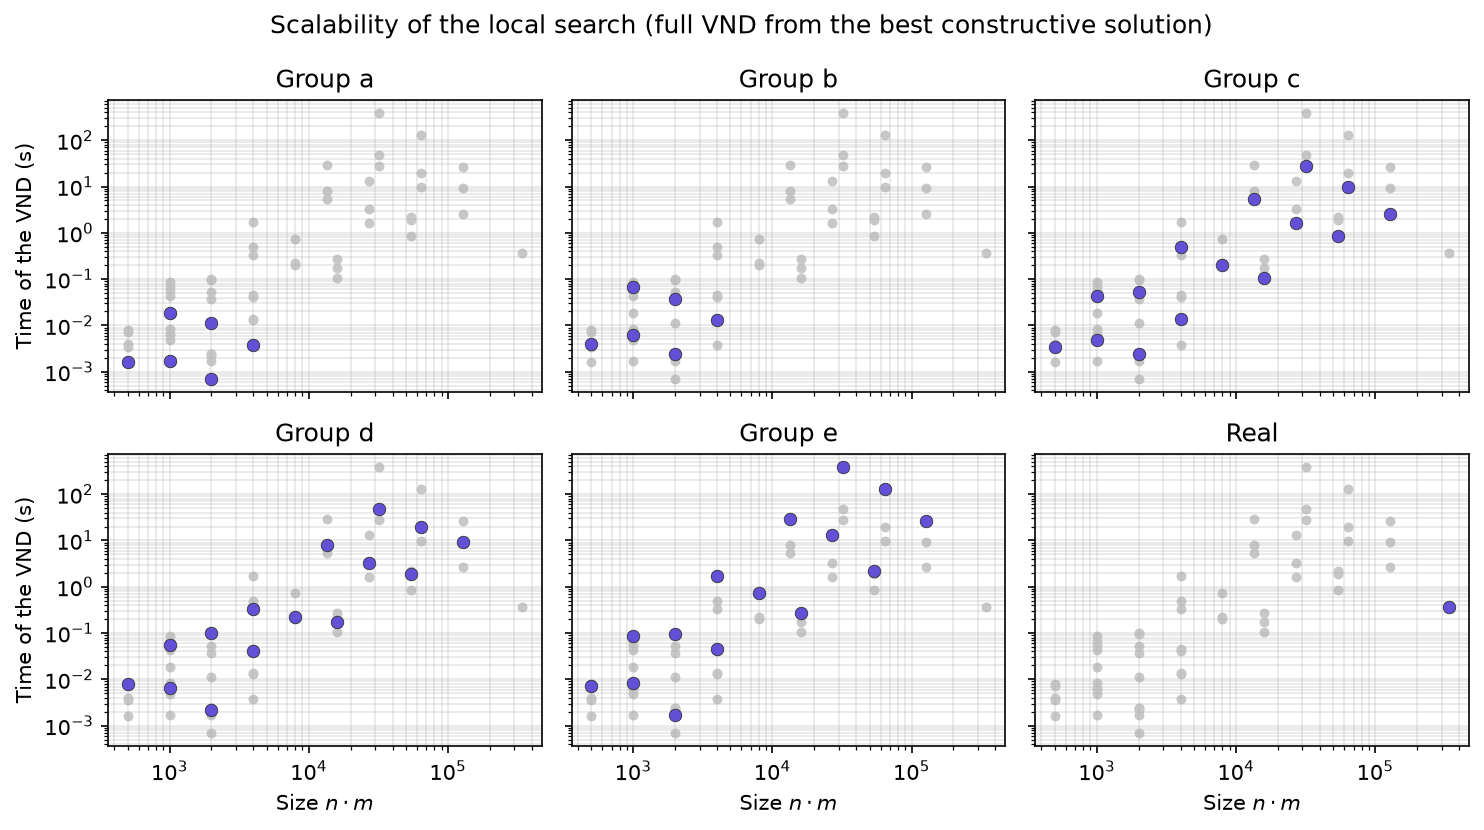
\includegraphics[width=\linewidth]{figs/fig_time_size.png}
  \caption{Time of the VND vs.\ size $n\cdot m$ (log-log).}\label{fig:tiempo}
\end{subfigure}
\caption{Summary of the final comparison: quality (gap) and scalability of the local search.}
\end{figure}

\subsection{E6 --- Real case: ThunderPack (RQ6)}
\begin{table}[ht]
\centering
\caption{Real instance ($m=310$, $n=1100$): cost, unassigned sellers, mean distance per assigned
seller and time, by method. Top, the heuristic chain (ILS and LNS: best of 5 seeds, and mean cost
in parentheses); bottom, the methods based on the relaxations.}
\label{tab:real}
\small
\begin{tabular}{l r r r r}
\toprule
Method & Cost & Unassigned & Mean distance & Time (s) \\
\midrule
Best constructive  & 718.0 & 0 & 0.65 & $<0.01$ \\
+ VND              & 695.5 & 0 & 0.63 & 0.15 \\
+ ILS              & 682.3 (683.4) & 0 & 0.62 & 60.0 \\
+ LNS              & 682.0 (682.4) & 0 & 0.62 & 60.0 \\
\midrule
Lagrangian heuristic + VND & 679.8 & 0 & 0.62 & $\approx3$ \\
MIP-LNS                    & \textbf{679.6} (679.6) & 0 & 0.62 & 60.0 \\
SCIP with fixing (optimum proven) & \textbf{679.6} & 0 & 0.62 & 8.8 \\
\bottomrule
\end{tabular}
\end{table}

\begin{figure}[ht]
\centering
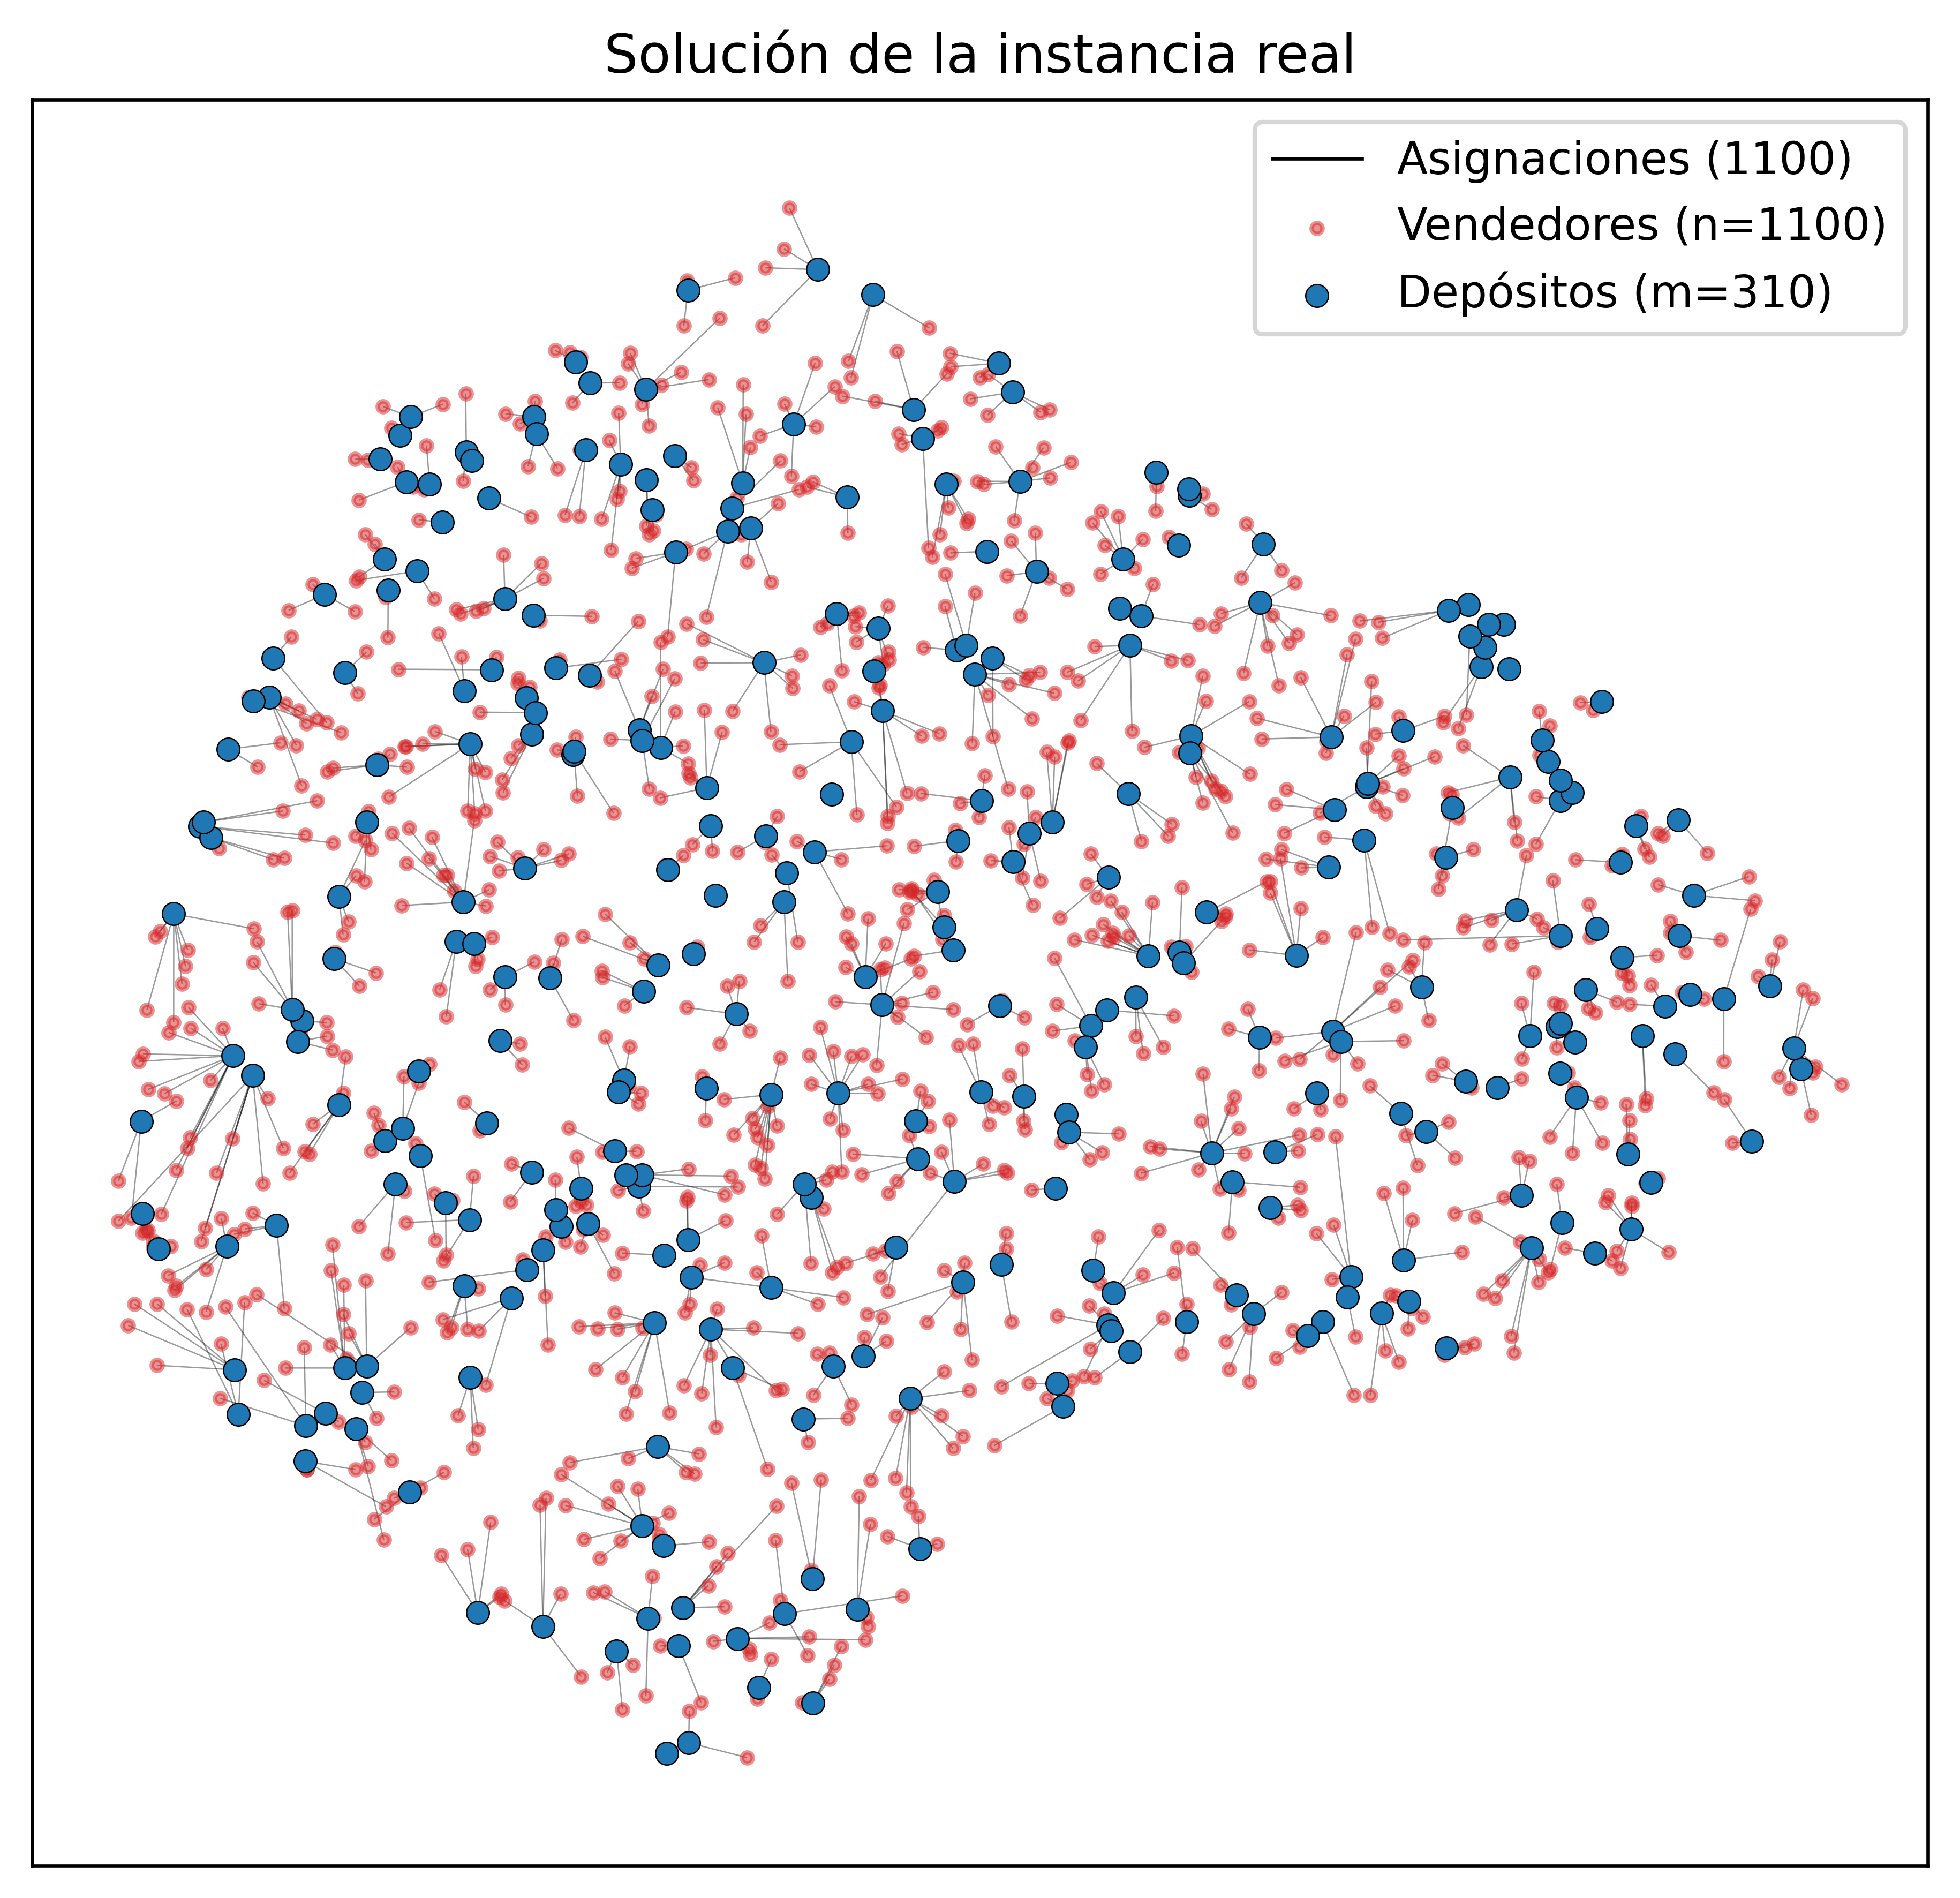
\includegraphics[width=0.55\linewidth]{figs/fig_map_real.png}
\caption{Geographic layout of the real instance ($n=1100$ sellers in red, $m=310$ warehouses in
blue). The gray lines join each seller with its warehouse in a heuristic solution of cost
$681.10$.}
\label{fig:mapa}
\end{figure}

\paragraph{Business reading (Q1--Q3).} The real instance is solved with 0 unassigned sellers by
every method: the aggregate capacity (ratio $0.70$) is enough and the geography does not prevent
it, so the network does not need to be expanded for the current demand (\textbf{Q1}; E15 measures
how much slack remains). The mean distance per seller goes down from $0.65$ (constructive) to
$0.62$ at the optimum: close and reasonable assignments (\textbf{Q2}). In time (\textbf{Q3}), the
constructive heuristic is instantaneous and the VND already cuts 3\,\% in $0.15$\,s; the Lagrangian
heuristic reaches $679.8$ in about 3\,s, $0.03\,\%$ from the optimum, and SCIP with fixing proves the
optimum, $679.60$, in $8.8$\,s. A one-hour run of the heuristic chain had reached $681.10$,
$0.22\,\%$ above it. An interactive tool can therefore deliver the optimal solution in seconds.

\subsection{Worst and best case (synthetic instances)}
To see in which cases each method fails or succeeds, besides the benchmark we built minimal
\emph{ad hoc} instances that trigger the worst and the best case of each kind of method.
Table~\ref{tab:sinteticas} summarizes what we observed.

\begin{table}[ht]
\centering
\caption{Worst/best case on synthetic instances. In each case, the cost that each method obtains
on the same instance.}
\label{tab:sinteticas}
\small
\begin{tabular}{@{}l l r l@{}}
\toprule
Case & Method & Cost & Interpretation \\
\midrule
\multirow{2}{*}{Myopic greedy}
  & Nearest neighbor & 101 & \emph{worst case} of the greedy \\
  & Regret insertion & 3   & \emph{best case} of the regret \\
\midrule
\multirow{2}{*}{3-cycle local optimum}
  & relocate + swap multiple & 30 & stuck (\emph{worst case} of 2 warehouses) \\
  & Full VND (cycle3) & 3 & escapes (\emph{best case} of the VND) \\
\midrule
\multirow{2}{*}{Metaheuristic}
  & ILS from a bad constructive & 3 & recovers the optimum (\emph{best case}) \\
  & ILS on an optimal instance & 2 & only \emph{overhead} (\emph{worst case}) \\
\bottomrule
\end{tabular}
\end{table}

In the \emph{myopic greedy} case, the nearest neighbor assigns the first seller to a warehouse that
the second one needed and ends at $101$, while the regret solves it at $3$. In the \emph{3-cycle
local optimum} we build an assignment that no \emph{relocate multiple} or \emph{swap multiple} (of
two warehouses) can leave, but the 3-warehouse \emph{cyclic exchange} of the VND can, and this
justifies that operator. Finally, the metaheuristic recovers the optimum from a very bad
constructive solution, but on an already optimal instance it cannot improve: what it gains depends
on how much room the local search leaves.

\subsection{E7--E10 --- Bounds, exact methods and true gaps (RQ7, RQ8)}
\emph{Hypothesis.} We expected the Lagrangian bound to be considerably better than the LP one, the
heuristics based on the relaxations to give good starting points, and the fixing to speed up SCIP a
lot, to the point of closing most instances in 600\,s.

\begin{table}[ht]
\centering
\caption{E7: mean distance (\%) of the LP bound and of the Lagrangian bound to the best known
bound, instances solved to optimality in 600\,s by SCIP, by SCIP with fixing and by the
branch-and-price with fixing (B\&P), and mean percentage of seller-warehouse pairs discarded by the
fixing.}
\label{tab:exact}
\small
\begin{tabular}{l r r r r r r r}
\toprule
 & & \multicolumn{2}{c}{Bound gap (\%)} & \multicolumn{3}{c}{Solved in 600\,s} & \\
\cmidrule(lr){3-4}\cmidrule(lr){5-7}
Group & Inst. & LP & Lagrangian & SCIP & SCIP + fix. & B\&P + fix. & \% discarded \\
\midrule
$a$ & 6 & 0.047 & 0.000 & 6 & 6 & 6 & 0.0 \\
$b$ & 6 & 0.483 & 0.063 & 6 & 6 & 6 & 32.9 \\
$c$ & 15 & 0.353 & 0.040 & 9 & 9 & 7 & 63.8 \\
$d$ & 15 & 0.095 & 0.022 & 1 & 0 & 2 & 0.0 \\
$e$ & 15 & 0.128 & 0.018 & 9 & 8 & 7 & 25.2 \\
\textbf{real} & 1 & 2.855 & 0.040 & 1 & 1 & 0 & 98.8 \\
\midrule
Total & 58 & & & 32 & 30 & 28 & \\
\bottomrule
\end{tabular}
\end{table}

\paragraph{Bounds and exact methods (E7).} The bounds behave as we expected
(Table~\ref{tab:exact}): the Lagrangian bound stays on average within $0.07\,\%$ of the best bound
in every group, several times closer than the LP one (on the real instance, $679.33$ against
$660.20$). The fixing, instead, depends on the starting solution. On the real instance it discards
$98.8\,\%$ of the pairs and SCIP goes from $88.6$ to $8.8$\,s. In $c$ and $e$ it discards between a
quarter and two thirds. In $d$ it discards nothing, even though the starting solution is not
farther from the bound than in $c$ or $e$ (between $0.2$ and $1.8\,\%$): on that type of instances
a solution much closer to the optimum is needed. For example, on \code{d05100}, with a solution of
$6388$ it discards nothing, with $6360$ it discards 34\,\% and with the optimum, $6353$, 64\,\%. In
group $a$ the 0\,\% has another cause: the bound already proves that the starting solution is
optimal. Together, the three methods solve 33 instances in 600\,s; type $d$ remains almost entirely
open.

\paragraph{Matheuristic (E8, E9).} To configure the MIP-LNS we tried 27 combinations of starting
point, destruction method and size on five instances (E8): the starting point weighed much more
than the rest. From the Lagrangian heuristic the mean gap stayed between $0.01$ and $1.1\,\%$ on all
five; from the best constructive solution it reached $234\,\%$ on \code{e15900}. We chose to start
from the Lagrangian heuristic and to destroy groups of nearby warehouses. In E9 we compared, with
the same budget, the LNS of E5, the same LNS started from the Lagrangian heuristic and the MIP-LNS
(Figure~\ref{fig:true_gaps}). Almost all the gain comes from the start: the LNS started from the
Lagrangian heuristic lowers the mean gap in $e$ from $125.6$ to $0.93\,\%$ and on the real instance
from $0.81$ to $0.015\,\%$. The MIP-LNS adds a smaller improvement: it is the best in $b$, $e$ and
the real one, where it finds the optimum with 4 of the 5 seeds, but in $d$ it falls slightly
behind.

\begin{figure}[ht]
\centering
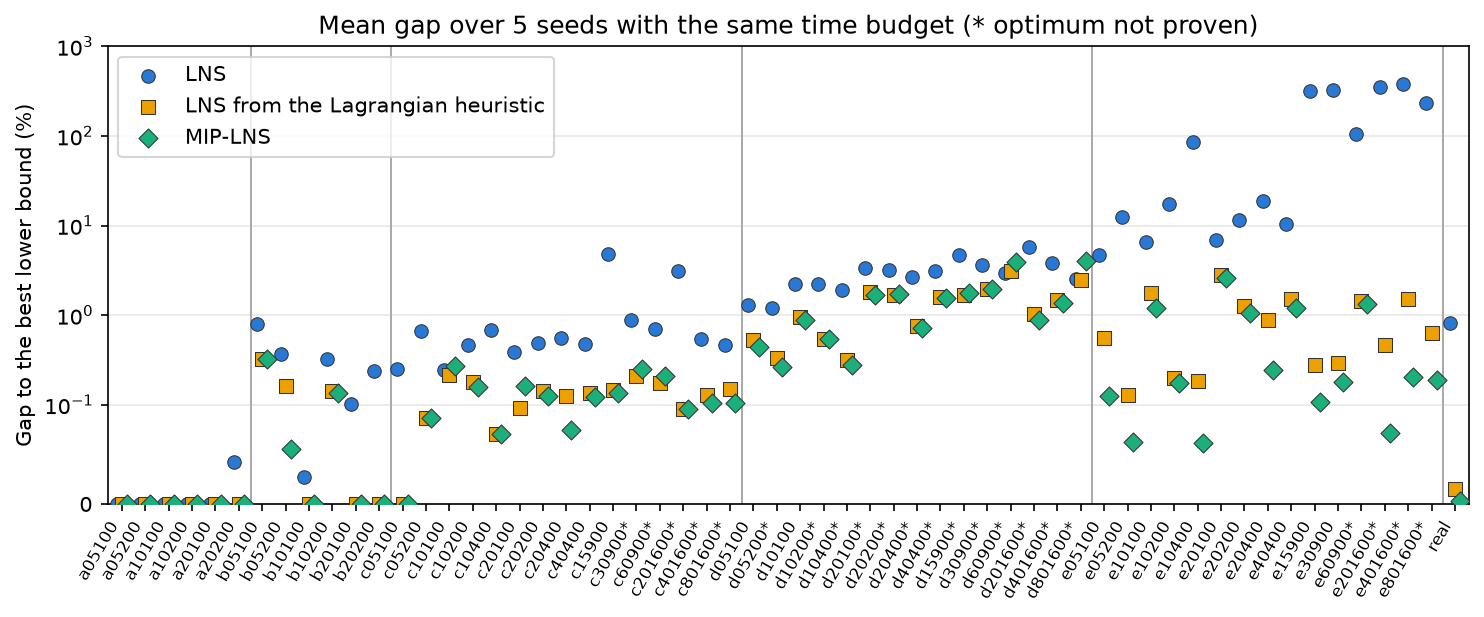
\includegraphics[width=\linewidth]{figs/fig_true_gaps.png}
\caption{E9: mean true gap (5 seeds, same budget) of the LNS, of the LNS started from the
Lagrangian heuristic and of the MIP-LNS, on the 58 instances (log scale; $*$: optimum not
proven).}
\label{fig:true_gaps}
\end{figure}

\begin{table}[ht]
\centering
\caption{E10: mean true gap (\%) of each method, by group, against the best known lower bound. In
the last row, instances with the optimum proven at the end of the work.}
\label{tab:gaps}
\small
\resizebox{\textwidth}{!}{%
\begin{tabular}{l r r r r r r r}
\toprule
Method & $a$ & $b$ & $c$ & $d$ & $e$ & real & All \\
\midrule
Best constructive & 0.01 & 52.92 & 109.15 & 66.36 & 691.59 & 5.65 & 229.82 \\
+ VND & 0.01 & 3.01 & 3.73 & 5.10 & 218.56 & 2.34 & 59.16 \\
ILS (mean) & 0.00 & 0.33 & 0.99 & 2.85 & 119.69 & 0.83 & 31.99 \\
LNS (mean) & 0.01 & 0.31 & 0.98 & 2.98 & 125.59 & 0.81 & 33.55 \\
\midrule
LP rounding + VND & 0.00 & 0.36 & 0.55 & 1.02 & 2.52 & 1.75 & 1.13 \\
Lagrangian heuristic + VND & 0.00 & 0.14 & 0.25 & 0.99 & 0.95 & 0.03 & 0.58 \\
LNS from the Lagrangian heuristic (mean) & 0.00 & 0.10 & 0.13 & 1.35 & 0.93 & 0.01 & 0.63 \\
MIP-LNS (mean) & 0.00 & 0.09 & 0.13 & 1.46 & 0.59 & 0.00 & 0.57 \\
\midrule
SCIP + fixing (600\,s) & 0.00 & 0.00 & 0.06 & 0.58 & 0.42 & 0.00 & 0.27 \\
Branch-and-price + fixing (600\,s) & 0.00 & 0.00 & 0.08 & 0.50 & 0.26 & 0.00 & 0.22 \\
\midrule
Optimum proven & 6/6 & 6/6 & 10/15 & 2/15 & 11/15 & 1/1 & 36/58 \\
\bottomrule
\end{tabular}%
}
\end{table}

\paragraph{True gaps (E10).} Table~\ref{tab:gaps} sums everything up. The metaheuristics of the
first stage stay within 1\,\% in $a$, $b$, $c$ and the real instance, but not in $d$ or $e$. The
heuristics based on the relaxations are much more even: the Lagrangian heuristic with VND, alone
and in a few seconds, stays on average at $0.58\,\%$, against $33.6\,\%$ for the LNS. The exact
methods, stopped at 600\,s, end within $0.6\,\%$ in every group. With all the experiments, the
optimum is proven on 36 of the 58 instances.

\subsection{E11--E12 --- Cutting planes and roundings (RQ9)}
\emph{Hypothesis.} We expected the cutting planes to bring the LP bound closer to the Lagrangian
one, and the rounding of Shmoys and Tardos, which has a cost guarantee, to give better solutions
than the simple rounding.

The first part holds only halfway. The cover inequalities close between 30 and 89\,\% of the
distance between the LP bound and the Lagrangian one, depending on the group, always less than the
cuts that SCIP adds on its own. The exact separation reaches the Lagrangian bound on almost every
instance of $b$ and $e$ and on the real one, but it takes up to the 600\,s of the limit and in $d$
it never finishes. The Lagrangian bound, instead, is computed in less than a minute (E14): for this
problem it is better than any family of cuts. The second part does not hold: the guarantee of
Shmoys and Tardos is verified on the 58 instances, but their assignment exceeds the capacity of
many warehouses (112 of 310 on the real one) and, after it is repaired, it is better than the simple
rounding on 25 instances and worse on 32. The simple rounding is enough.

\subsection{E13--E14 --- The branch-and-price (RQ10)}
\emph{Hypothesis.} We expected the speed-up techniques of the branch-and-price to help, and a better
solver for the linear program of the root to let it advance on the large instances.

On eight small instances that the branch-and-price solves, switching off each technique one at a
time does not change how many it solves, and the version without any of them is the fastest
(15\,s against 30\,s; E13): on instances of this size, the techniques cost more than they save.
The problem lies in the large ones (E14, Figure~\ref{fig:master}): neither the simplex nor the
interior point method of HiGHS finishes the linear program of the root in 300\,s on four of eight
instances, the real one included. The bundle method, instead, computes the same bound on 57 of the
58 instances in a median of half a second and in at most 38\,s (on the remaining one it stays
$0.004$ from the exact value). Even so, the branch-and-price needs the solution of the linear
program to branch, so on the instances with 900 sellers or more it barely gets past the root: on
almost all of them it explores one or two nodes in 600\,s (E17).

\begin{figure}[ht]
\centering
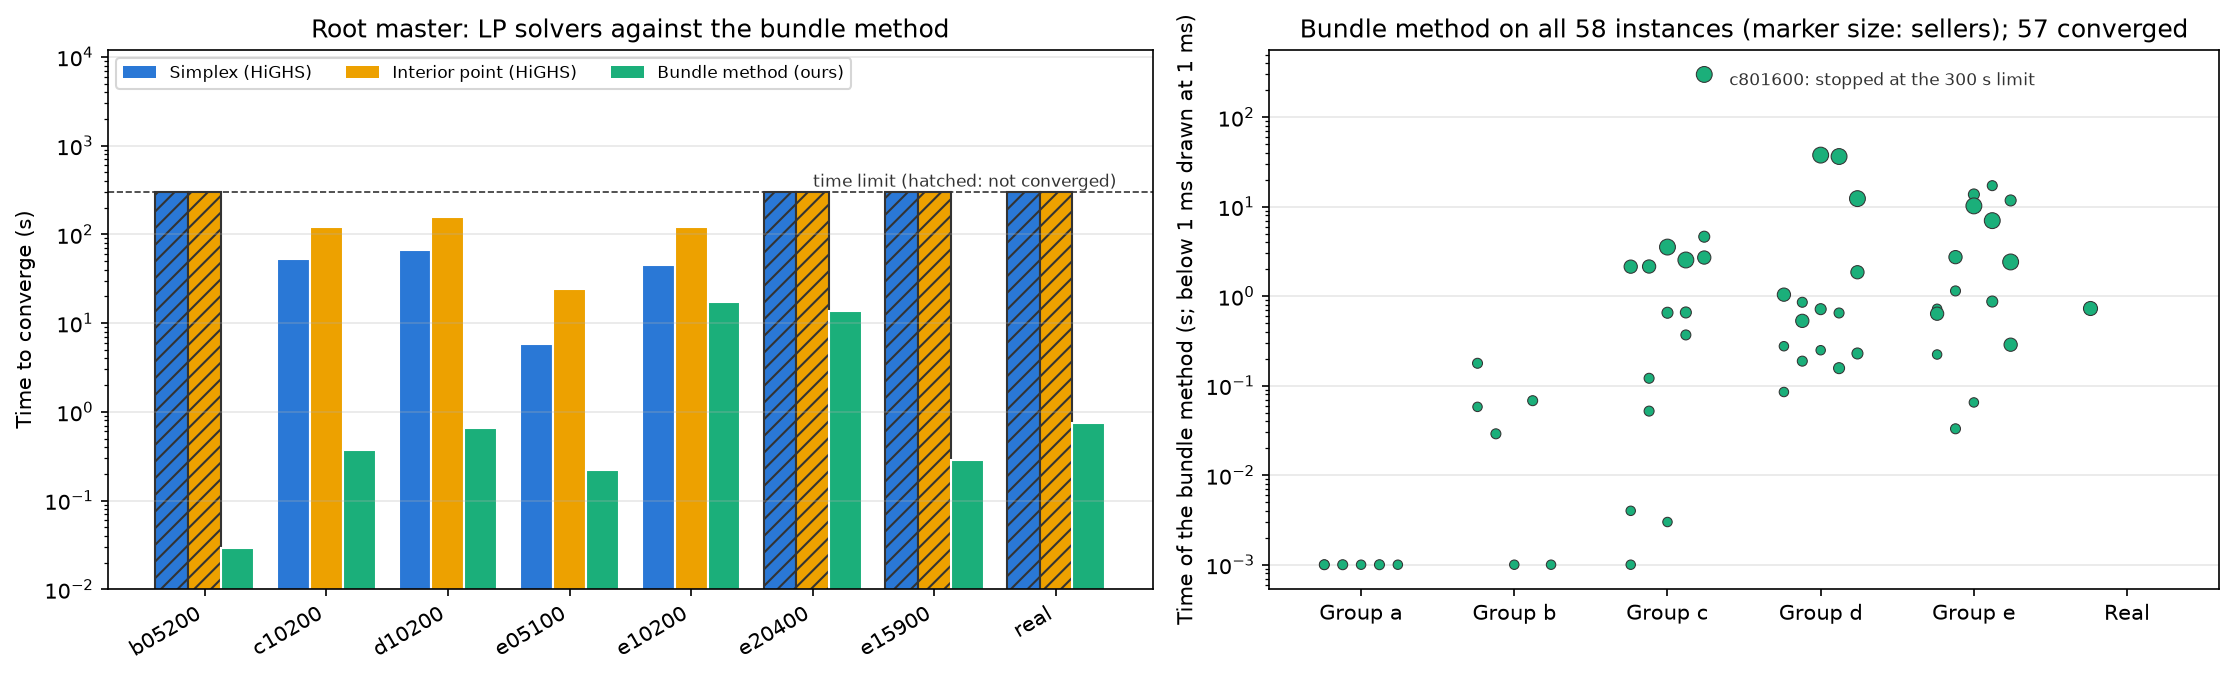
\includegraphics[width=\linewidth]{figs/fig_master.png}
\caption{E14: left, time to compute the bound of the root with the simplex, the interior point
method and the bundle method (hatched: did not finish in 300\,s); right, time of the bundle method
on the 58 instances, by group (marker size: number of sellers).}
\label{fig:master}
\end{figure}

\subsection{E15 --- Slack of the real network (RQ11)}
\emph{Hypothesis.} We expected the shadow prices of the capacities (how much the cost goes down
per unit of extra capacity, according to the LP) to estimate well the saving of expanding a
warehouse, and closing a heavily loaded one to cost a lot.

Starting from the optimum, we solved the real instance again in three kinds of scenarios: 10 more
units of capacity in each of the 15 warehouses with the largest shadow price, the closure of each
of the 15 most loaded warehouses and an increase of the demand (Figure~\ref{fig:sens}).

\begin{figure}[ht]
\centering
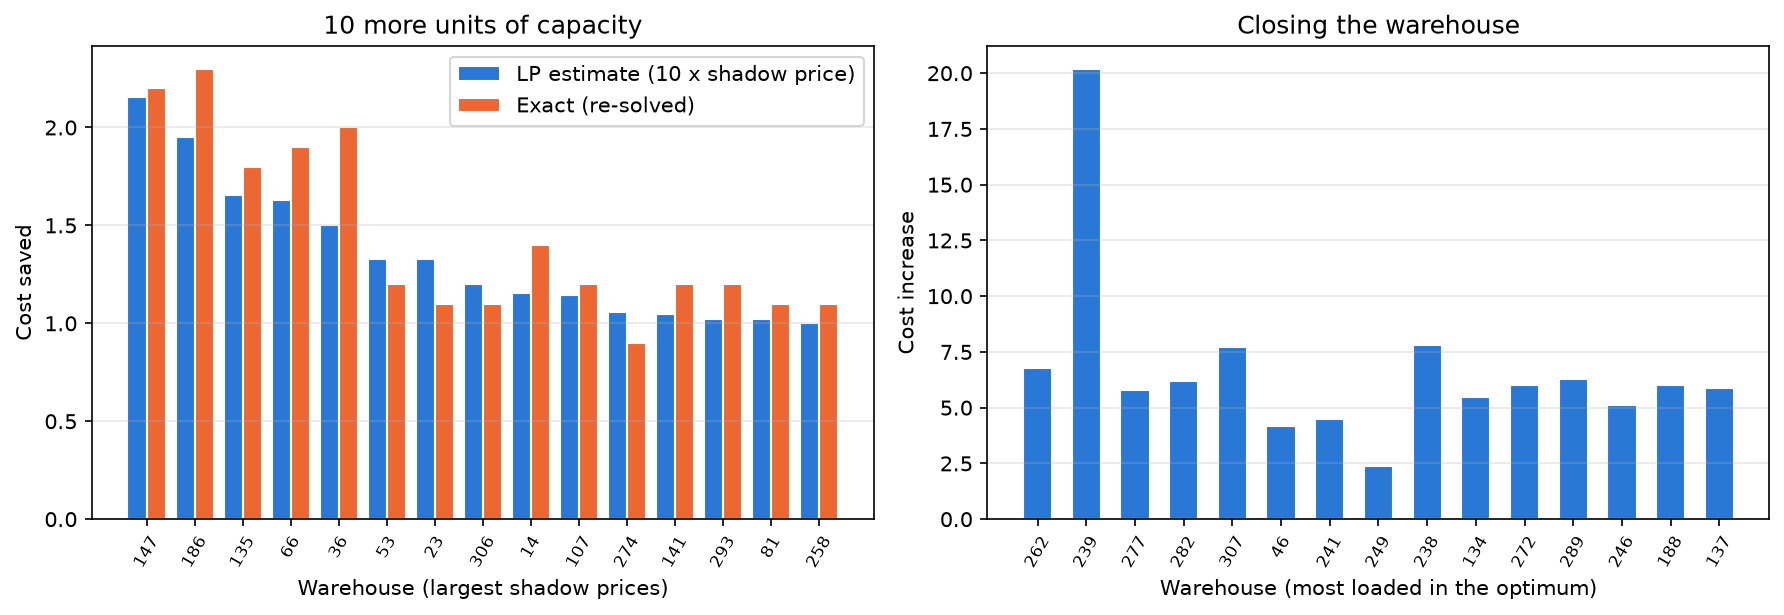
\includegraphics[width=\linewidth]{figs/fig_sensitivity.png}
\caption{E15: left, saving of 10 more units of capacity in the 15 warehouses with the largest
shadow price, estimated by the LP and exact; right, cost increase when closing each of the 15 most
loaded warehouses.}
\label{fig:sens}
\end{figure}

The shadow price estimates the saving well: between $0.9$ and $2.3$ per 10 units, at most
$0.34\,\%$ of the cost, so expanding one warehouse does not change the picture. Closing one of the
most loaded warehouses costs between $2.4$ and $20.2$ (between $0.4$ and 3\,\%), always without
leaving sellers out; the most critical one is warehouse 239, whose closure costs $20.2$ although its
shadow price is only $0.08$, so the shadow price does not anticipate the cost of a closure. For the
demand we multiplied each one by $1.05$, $1.10$ and $1.20$, rounding up; since the demands are small
integers, the total demand actually grows by 10, 14 and 24\,\%. Even so, every seller fits, with
costs of $721.9$, $744.9$ and $818.4$.

\subsection{E16--E17 --- The open instances (RQ12)}
\emph{Hypothesis.} Since the fixing did not work on $d$, we expected that starting from better
solutions and re-fixing during the search would close a good number of the open instances.

In E16, on the 30 instances that the fixing of E7 does not close in 100\,s, re-fixing doubled the
instances solved in 300\,s (from 2 to 4), and starting from the MIP-LNS gave the lowest mean gap
($0.33\,\%$), but no variant solved more than 4. On the large type-$d$ instances, 60\,s of MIP-LNS
even gave worse solutions than those of E7. That is why in E17 we tried, on the 24 instances still
open, four heuristics with 120\,s (Table~\ref{tab:open}) and, from the solution of the portfolio,
SCIP and the branch-and-price with re-fixing for 600\,s.

\begin{table}[ht]
\centering
\caption{E17: mean true gap (\%) of each heuristic with 120\,s on the 24 open instances, by group,
and instances on which it is the best (ties included).}
\label{tab:open}
\small
\begin{tabular}{l r r r r r}
\toprule
Heuristic (120\,s) & $c$ (5) & $d$ (13) & $e$ (6) & All & Best on \\
\midrule
MIP-LNS                         & 0.149 & 0.698 & \textbf{0.122} & 0.440 & 9 \\
Tabu search                     & 0.141 & 1.323 & 1.390 & 1.094 & 0 \\
LP rounding + MIP-LNS           & 0.153 & 0.478 & 0.223 & 0.346 & 4 \\
Portfolio                       & \textbf{0.099} & \textbf{0.426} & 0.148 & \textbf{0.288} & 12 \\
\bottomrule
\end{tabular}
\end{table}

The hypothesis holds only in part. The portfolio was the best heuristic on average, and with E17
the best known solution went down on 18 of the 24 instances. With that, the fixing started to work
where the solution ended up very close to the optimum: SCIP with re-fixing closed \code{e40400} and
\code{e30900}, while the discarded pairs went up from 45 to 90\,\% and from 51 to 95\,\%. In type
$d$ it only worked on the two instances that ended up closest to the optimum (\code{d05200} and
\code{d20100}, $0.05\,\%$ from the bound, where it discarded 42 and 50\,\% of the pairs); on the
others, the remaining distance (between $0.1$ and $0.9\,\%$) is still too large. 22 instances remain
open (5 of $c$, 13 of $d$ and 4 of $e$), all with a gap below 1\,\%.

%==============================================================================
\section{Conclusions}\label{sec:concl}
%==============================================================================
\begin{itemize}
  \item \textbf{Answer to Q1--Q3 (real case).} The optimum of the real instance is $679.60$, with
        every seller assigned: the current network is enough (\textbf{Q1}) and has slack to spare,
        since it absorbs 24\,\% more demand without leaving anyone out and the closure of any of
        the 15 most loaded warehouses costs at most 3\,\% (E15). The mean distance is $0.62$ per
        seller (\textbf{Q2}). The Lagrangian heuristic gives, in about 3\,s, a solution $0.03\,\%$
        from the optimum, and SCIP with fixing proves the optimum in $8.8$\,s (\textbf{Q3}): such a
        tool can be used in real time.
  \item \textbf{Measuring against a bound changes the reading.} Compared only with each other, the
        metaheuristics did not exceed a 9\,\% mean gap in any group; against the lower bound they
        stay around 3\,\% from the optimum in $d$ and above 100\,\% in $e$.
  \item \textbf{The relaxations give the best starting points.} The Lagrangian heuristic with VND
        stays, alone, at $0.58\,\%$ on average, and the LNS or the MIP-LNS started from it, within
        1\,\% in every group except $d$. The start weighs more than the rest of the configuration.
  \item \textbf{The Lagrangian bound is the central tool.} It is better than the LP bound and than
        that of the cutting planes, and it allows discarding almost the whole problem when the
        known solution is close to the optimum (on the real instance, $98.8\,\%$ of the pairs).
  \item \textbf{What remains open.} Type $d$, with very tight capacities, is by far the hardest: 13
        of its 15 instances are still open, all with a gap below 1\,\%. The next steps would be to
        let the branch-and-price branch without solving the linear program of the root, and a more
        complete tabu search for that type of instances.
\end{itemize}

%==============================================================================
\begin{thebibliography}{99}
\small
\setlength{\itemsep}{0pt}
\bibitem{avella2010} P.~Avella, M.~Boccia and I.~Vasilyev. A computational study of exact knapsack
  separation for the generalized assignment problem. \emph{Computational Optimization and
  Applications}, 45(3):543--555, 2010.
\bibitem{beasley1990} J.~E. Beasley. OR-Library: distributing test problems by electronic mail.
  \emph{Journal of the Operational Research Society}, 41(11):1069--1072, 1990.
\bibitem{benders1983} J.~F. Benders and J.~A.~E.~E. van Nunen. A property of assignment type mixed
  integer linear programming problems. \emph{Operations Research Letters}, 2(2):47--52, 1983.
\bibitem{briant2008} O.~Briant, C.~Lemaréchal, Ph.~Meurdesoif, S.~Michel, N.~Perrot and
  F.~Vanderbeck. Comparison of bundle and classical column generation. \emph{Mathematical
  Programming}, 113(2):299--344, 2008.
\bibitem{fisher1986} M.~L. Fisher, R.~Jaikumar and L.~N. Van Wassenhove. A multiplier adjustment
  method for the generalized assignment problem. \emph{Management Science}, 32(9):1095--1103,
  1986.
\bibitem{highs} Q.~Huangfu and J.~A.~J. Hall. Parallelizing the dual revised simplex method.
  \emph{Mathematical Programming Computation}, 10(1):119--142, 2018. (HiGHS, \url{https://highs.dev}).
\bibitem{martello1981} S.~Martello and P.~Toth. An algorithm for the generalized assignment
  problem. In J.~P. Brans (ed.), \emph{Operational Research '81}, 589--603. North-Holland, 1981.
\bibitem{posta2012} M.~Posta, J.~A. Ferland and P.~Michelon. An exact method with variable fixing
  for solving the generalized assignment problem. \emph{Computational Optimization and
  Applications}, 52(3):629--644, 2012.
\bibitem{savelsbergh1997} M.~Savelsbergh. A branch-and-price algorithm for the generalized
  assignment problem. \emph{Operations Research}, 45(6):831--841, 1997.
\bibitem{scip} SCIP Optimization Suite, version 10.1. \url{https://www.scipopt.org}.
\bibitem{shmoys1993} D.~B. Shmoys and É.~Tardos. An approximation algorithm for the generalized
  assignment problem. \emph{Mathematical Programming}, 62:461--474, 1993.
\bibitem{yagiura2004} M.~Yagiura, T.~Ibaraki and F.~Glover. An ejection chain approach for the
  generalized assignment problem. \emph{INFORMS Journal on Computing}, 16(2):133--151, 2004.
\end{thebibliography}

%==============================================================================
\appendix
\section{Results per instance}\label{sec:apendice}
%==============================================================================
\begin{table}[H]
\centering
\caption{Best lower bound and best solution of each instance at the end of the work, whether the
optimum is proven, its gap (\%) and the mean true gap (5 seeds) of the LNS (E5) and of the MIP-LNS
(E9).}
\label{tab:apendice}
\scriptsize
\begin{tabular}{l r r r r c r r r}
\toprule
Instance & $m$ & $n$ & Lower bound & Best solution & Optimum & Gap (\%) & LNS (\%) & MIP-LNS (\%) \\
\midrule
a05100 & 5 & 100 & 1,698 & 1,698 & yes & 0.000 & 0.00 & 0.00 \\
a05200 & 5 & 200 & 3,235 & 3,235 & yes & 0.000 & 0.00 & 0.00 \\
a10100 & 10 & 100 & 1,360 & 1,360 & yes & 0.000 & 0.00 & 0.00 \\
a10200 & 10 & 200 & 2,623 & 2,623 & yes & 0.000 & 0.00 & 0.00 \\
a20100 & 20 & 100 & 1,158 & 1,158 & yes & 0.000 & 0.00 & 0.00 \\
a20200 & 20 & 200 & 2,339 & 2,339 & yes & 0.000 & 0.04 & 0.00 \\
\midrule
b05100 & 5 & 100 & 1,843 & 1,843 & yes & 0.000 & 0.79 & 0.33 \\
b05200 & 5 & 200 & 3,552 & 3,552 & yes & 0.000 & 0.37 & 0.06 \\
b10100 & 10 & 100 & 1,407 & 1,407 & yes & 0.000 & 0.03 & 0.00 \\
b10200 & 10 & 200 & 2,827 & 2,827 & yes & 0.000 & 0.33 & 0.13 \\
b20100 & 20 & 100 & 1,166 & 1,166 & yes & 0.000 & 0.10 & 0.00 \\
b20200 & 20 & 200 & 2,339 & 2,339 & yes & 0.000 & 0.24 & 0.00 \\
\midrule
c05100 & 5 & 100 & 1,931 & 1,931 & yes & 0.000 & 0.25 & 0.00 \\
c05200 & 5 & 200 & 3,456 & 3,456 & yes & 0.000 & 0.66 & 0.09 \\
c10100 & 10 & 100 & 1,402 & 1,402 & yes & 0.000 & 0.24 & 0.27 \\
c10200 & 10 & 200 & 2,806 & 2,806 & yes & 0.000 & 0.46 & 0.16 \\
c10400 & 10 & 400 & 5,597 & 5,597 & yes & 0.000 & 0.69 & 0.07 \\
c20100 & 20 & 100 & 1,243 & 1,243 & yes & 0.000 & 0.39 & 0.16 \\
c20200 & 20 & 200 & 2,391 & 2,391 & yes & 0.000 & 0.48 & 0.12 \\
c20400 & 20 & 400 & 4,782 & 4,782 & yes & 0.000 & 0.56 & 0.07 \\
c40400 & 40 & 400 & 4,244 & 4,244 & yes & 0.000 & 0.47 & 0.12 \\
c15900 & 15 & 900 & 11,340 & 11,340 & yes & 0.000 & 4.78 & 0.14 \\
c30900 & 30 & 900 & 9,982 & 9,985 & no & 0.030 & 0.87 & 0.25 \\
c60900 & 60 & 900 & 9,325 & 9,334 & no & 0.097 & 0.69 & 0.21 \\
c201600 & 20 & 1600 & 18,802 & 18,807 & no & 0.027 & 3.10 & 0.10 \\
c401600 & 40 & 1600 & 17,144 & 17,153 & no & 0.052 & 0.55 & 0.11 \\
c801600 & 80 & 1600 & 16,284 & 16,296 & no & 0.074 & 0.46 & 0.11 \\
\midrule
d05100 & 5 & 100 & 6,353 & 6,353 & yes & 0.000 & 1.30 & 0.44 \\
d05200 & 5 & 200 & 12,741 & 12,747 & no & 0.047 & 1.22 & 0.26 \\
d10100 & 10 & 100 & 6,347 & 6,347 & yes & 0.000 & 2.23 & 0.89 \\
d10200 & 10 & 200 & 12,428 & 12,444 & no & 0.129 & 2.23 & 0.54 \\
d10400 & 10 & 400 & 24,959 & 24,983 & no & 0.096 & 1.93 & 0.28 \\
d20100 & 20 & 100 & 6,182 & 6,185 & no & 0.049 & 3.33 & 1.67 \\
d20200 & 20 & 200 & 12,232 & 12,312 & no & 0.654 & 3.21 & 1.72 \\
d20400 & 20 & 400 & 24,561 & 24,638 & no & 0.314 & 2.67 & 0.71 \\
d40400 & 40 & 400 & 24,350 & 24,578 & no & 0.936 & 3.15 & 1.54 \\
d15900 & 15 & 900 & 55,403 & 55,476 & no & 0.132 & 4.64 & 1.77 \\
d30900 & 30 & 900 & 54,833 & 54,983 & no & 0.274 & 3.63 & 1.96 \\
d60900 & 60 & 900 & 54,551 & 54,884 & no & 0.610 & 2.96 & 3.88 \\
d201600 & 20 & 1600 & 97,823 & 97,923 & no & 0.102 & 5.77 & 0.89 \\
d401600 & 40 & 1600 & 97,105 & 97,450 & no & 0.355 & 3.82 & 1.35 \\
d801600 & 80 & 1600 & 97,034 & 97,579 & no & 0.562 & 2.56 & 3.98 \\
\midrule
e05100 & 5 & 100 & 12,681 & 12,681 & yes & 0.000 & 4.72 & 0.13 \\
e05200 & 5 & 200 & 24,930 & 24,930 & yes & 0.000 & 12.58 & 0.06 \\
e10100 & 10 & 100 & 11,577 & 11,577 & yes & 0.000 & 6.55 & 1.20 \\
e10200 & 10 & 200 & 23,307 & 23,307 & yes & 0.000 & 17.16 & 0.17 \\
e10400 & 10 & 400 & 45,746 & 45,746 & yes & 0.000 & 85.18 & 0.06 \\
e20100 & 20 & 100 & 8,436 & 8,436 & yes & 0.000 & 6.91 & 2.62 \\
e20200 & 20 & 200 & 22,379 & 22,379 & yes & 0.000 & 11.44 & 1.07 \\
e20400 & 20 & 400 & 44,877 & 44,877 & yes & 0.000 & 19.01 & 0.24 \\
e40400 & 40 & 400 & 44,561 & 44,561 & yes & 0.000 & 10.52 & 1.20 \\
e15900 & 15 & 900 & 102,421 & 102,421 & yes & 0.000 & 313.25 & 0.11 \\
e30900 & 30 & 900 & 100,427 & 100,427 & yes & 0.000 & 324.31 & 0.18 \\
e60900 & 60 & 900 & 100,147 & 100,331 & no & 0.184 & 105.37 & 1.33 \\
e201600 & 20 & 1600 & 180,644 & 180,727 & no & 0.046 & 351.54 & 0.07 \\
e401600 & 40 & 1600 & 178,293 & 178,516 & no & 0.125 & 380.77 & 0.20 \\
e801600 & 80 & 1600 & 176,819 & 177,059 & no & 0.136 & 234.58 & 0.19 \\
\midrule
\textbf{real} & 310 & 1100 & 679.60 & 679.60 & yes & 0.000 & 0.81 & 0.00 \\
\bottomrule
\end{tabular}
\end{table}

\end{document}
